\documentclass[a4paper,12pt,twoside]{memoir}

% Castellano
\usepackage[spanish,es-tabla]{babel}
\selectlanguage{spanish}
\usepackage[utf8]{inputenc}
\usepackage[T1]{fontenc}
\usepackage{lmodern} % scalable font
\usepackage{microtype}
\usepackage{placeins}

\RequirePackage{booktabs}
\RequirePackage[table]{xcolor}
\RequirePackage{xtab}
\RequirePackage{multirow}

% Links
\PassOptionsToPackage{hyphens}{url}\usepackage[colorlinks]{hyperref}
\hypersetup{
	allcolors = {red}
}

% Ecuaciones
\usepackage{amsmath}

% Rutas de fichero / paquete
\newcommand{\ruta}[1]{{\sffamily #1}}

% Párrafos
\nonzeroparskip

% Huérfanas y viudas
\widowpenalty100000
\clubpenalty100000

% Evitar solapes en el header
\nouppercaseheads

% Imagenes
\usepackage{graphicx}
\newcommand{\imagen}[2]{
	\begin{figure}[!h]
		\centering
		\includegraphics[width=0.9\textwidth]{#1}
		\caption{#2}\label{fig:#1}
	\end{figure}
	\FloatBarrier
}

\newcommand{\imagenflotante}[2]{
	\begin{figure}%[!h]
		\centering
		\includegraphics[width=0.9\textwidth]{#1}
		\caption{#2}\label{fig:#1}
	\end{figure}
}



% El comando \figura nos permite insertar figuras comodamente, y utilizando
% siempre el mismo formato. Los parametros son:
% 1 -> Porcentaje del ancho de página que ocupará la figura (de 0 a 1)
% 2 --> Fichero de la imagen
% 3 --> Texto a pie de imagen
% 4 --> Etiqueta (label) para referencias
% 5 --> Opciones que queramos pasarle al \includegraphics
% 6 --> Opciones de posicionamiento a pasarle a \begin{figure}
\newcommand{\figuraConPosicion}[6]{%
  \setlength{\anchoFloat}{#1\textwidth}%
  \addtolength{\anchoFloat}{-4\fboxsep}%
  \setlength{\anchoFigura}{\anchoFloat}%
  \begin{figure}[#6]
    \begin{center}%
      \Ovalbox{%
        \begin{minipage}{\anchoFloat}%
          \begin{center}%
            \includegraphics[width=\anchoFigura,#5]{#2}%
            \caption{#3}%
            \label{#4}%
          \end{center}%
        \end{minipage}
      }%
    \end{center}%
  \end{figure}%
}

%
% Comando para incluir imágenes en formato apaisado (sin marco).
\newcommand{\figuraApaisadaSinMarco}[5]{%
  \begin{figure}%
    \begin{center}%
    \includegraphics[angle=90,height=#1\textheight,#5]{#2}%
    \caption{#3}%
    \label{#4}%
    \end{center}%
  \end{figure}%
}
% Para las tablas
\newcommand{\otoprule}{\midrule [\heavyrulewidth]}
%
% Nuevo comando para tablas pequeñas (menos de una página).
\newcommand{\tablaSmall}[5]{%
 \begin{table}
  \begin{center}
   \rowcolors {2}{gray!35}{}
   \begin{tabular}{#2}
    \toprule
    #4
    \otoprule
    #5
    \bottomrule
   \end{tabular}
   \caption{#1}
   \label{tabla:#3}
  \end{center}
 \end{table}
}

%
%Para el float H de tablaSmallSinColores
\usepackage{float}

%
% Nuevo comando para tablas pequeñas (menos de una página).
\newcommand{\tablaSmallSinColores}[5]{%
 \begin{table}[H]
  \begin{center}
   \begin{tabular}{#2}
    \toprule
    #4
    \otoprule
    #5
    \bottomrule
   \end{tabular}
   \caption{#1}
   \label{tabla:#3}
  \end{center}
 \end{table}
}

\newcommand{\tablaApaisadaSmall}[5]{%
\begin{landscape}
  \begin{table}
   \begin{center}
    \rowcolors {2}{gray!35}{}
    \begin{tabular}{#2}
     \toprule
     #4
     \otoprule
     #5
     \bottomrule
    \end{tabular}
    \caption{#1}
    \label{tabla:#3}
   \end{center}
  \end{table}
\end{landscape}
}

%
% Nuevo comando para tablas grandes con cabecera y filas alternas coloreadas en gris.
\newcommand{\tabla}[6]{%
  \begin{center}
    \tablefirsthead{
      \toprule
      #5
      \otoprule
    }
    \tablehead{
      \multicolumn{#3}{l}{\small\sl continúa desde la página anterior}\\
      \toprule
      #5
      \otoprule
    }
    \tabletail{
      \hline
      \multicolumn{#3}{r}{\small\sl continúa en la página siguiente}\\
    }
    \tablelasttail{
      \hline
    }
    \bottomcaption{#1}
    \rowcolors {2}{gray!35}{}
    \begin{xtabular}{#2}
      #6
      \bottomrule
    \end{xtabular}
    \label{tabla:#4}
  \end{center}
}

%
% Nuevo comando para tablas grandes con cabecera.
\newcommand{\tablaSinColores}[6]{%
  \begin{center}
    \tablefirsthead{
      \toprule
      #5
      \otoprule
    }
    \tablehead{
      \multicolumn{#3}{l}{\small\sl continúa desde la página anterior}\\
      \toprule
      #5
      \otoprule
    }
    \tabletail{
      \hline
      \multicolumn{#3}{r}{\small\sl continúa en la página siguiente}\\
    }
    \tablelasttail{
      \hline
    }
    \bottomcaption{#1}
    \begin{xtabular}{#2}
      #6
      \bottomrule
    \end{xtabular}
    \label{tabla:#4}
  \end{center}
}

%
% Nuevo comando para tablas grandes sin cabecera.
\newcommand{\tablaSinCabecera}[5]{%
  \begin{center}
    \tablefirsthead{
      \toprule
    }
    \tablehead{
      \multicolumn{#3}{l}{\small\sl continúa desde la página anterior}\\
      \hline
    }
    \tabletail{
      \hline
      \multicolumn{#3}{r}{\small\sl continúa en la página siguiente}\\
    }
    \tablelasttail{
      \hline
    }
    \bottomcaption{#1}
  \begin{xtabular}{#2}
    #5
   \bottomrule
  \end{xtabular}
  \label{tabla:#4}
  \end{center}
}



\definecolor{cgoLight}{HTML}{EEEEEE}
\definecolor{cgoExtralight}{HTML}{FFFFFF}

%
% Nuevo comando para tablas grandes sin cabecera.
\newcommand{\tablaSinCabeceraConBandas}[5]{%
  \begin{center}
    \tablefirsthead{
      \toprule
    }
    \tablehead{
      \multicolumn{#3}{l}{\small\sl continúa desde la página anterior}\\
      \hline
    }
    \tabletail{
      \hline
      \multicolumn{#3}{r}{\small\sl continúa en la página siguiente}\\
    }
    \tablelasttail{
      \hline
    }
    \bottomcaption{#1}
    \rowcolors[]{1}{cgoExtralight}{cgoLight}

  \begin{xtabular}{#2}
    #5
   \bottomrule
  \end{xtabular}
  \label{tabla:#4}
  \end{center}
}




\graphicspath{ {./img/} }

% Capítulos
\chapterstyle{bianchi}
\newcommand{\capitulo}[2]{
	\setcounter{chapter}{#1}
	\setcounter{section}{0}
	\setcounter{figure}{0}
	\setcounter{table}{0}
	\chapter*{#2}
	\addcontentsline{toc}{chapter}{#2}
	\markboth{#2}{#2}
}

% Apéndices
\renewcommand{\appendixname}{Apéndice}
\renewcommand*\cftappendixname{\appendixname}

\newcommand{\apendice}[1]{
	%\renewcommand{\thechapter}{A}
	\chapter{#1}
}

\renewcommand*\cftappendixname{\appendixname\ }

% Formato de portada
\makeatletter
\usepackage{xcolor}
\newcommand{\tutor}[1]{\def\@tutor{#1}}
\newcommand{\course}[1]{\def\@course{#1}}
\definecolor{cpardoBox}{HTML}{E6E6FF}
\def\maketitle{
  \null
  \thispagestyle{empty}
  % Cabecera ----------------
\noindent
\includegraphics[width=\textwidth]{cabecera}\vspace{1cm}%
  \vfill
  % Título proyecto y escudo informática ----------------
  \colorbox{cpardoBox}{%
    \begin{minipage}{.8\textwidth}
      \vspace{.5cm}\Large
      \begin{center}
      \textbf{TFG del Grado en Ingeniería Informática}\vspace{.6cm}\\
      \textbf{\LARGE\@title{}}
      \end{center}
      \vspace{.2cm}
    \end{minipage}

  }%
  \hfill\begin{minipage}{.20\textwidth}
    
\includegraphics[width=\textwidth]{escudoInfor}
  \end{minipage}
  \vfill
  % Datos de alumno, curso y tutores ------------------
  \begin{center}%
  {%
    \noindent\LARGE
    Presentado por \@author{}\\ 
    en Universidad de Burgos --- \@date{}\\
    Tutor: \@tutor{}\\
  }%
  \end{center}%
  \null
  \cleardoublepage
  }
\makeatother


% Datos de portada
\title{título del TFG \\Documentación Técnica}
\author{nombre alumno}
\tutor{nombre tutor}
\date{\today}

\begin{document}

\maketitle



\cleardoublepage



%%%%%%%%%%%%%%%%%%%%%%%%%%%%%%%%%%%%%%%%%%%%%%%%%%%%%%%%%%%%%%%%%%%%%%%%%%%%%%%%%%%%%%%%



\frontmatter


\clearpage

% Indices
\tableofcontents

\clearpage

\listoffigures

\clearpage

\listoftables

\clearpage

\mainmatter

\appendix

\apendice{Plan de Proyecto Software}
\label{apendice:plan_proyecto}

\section{Introducción}
\label{sec:plan_intro}

La planificación de un proyecto es una fase fundamental para su correcto desarrollo. En este apartado se comentará, por una parte, la planificación temporal del proyecto mediante los distintos \textit{sprints} que se han llevado a cabo, y por otra parte, se realizará un breve estudio sobre la viabilidad del proyecto.

En este proyecto se ha utilizado una metodología ágil basada en los principios de \textit{Scrum}, que tiene como objetivo base la creación de diferentes iteraciones o \textbf{sprints} \cite{trigas2012metodologia}. Para una correcta planificación, se optó por agrupar el trabajo en Épicas que contienen Sprints con objetivos temáticos, gestionando todas las tareas a través de un tablero en la plataforma \textbf{Jira}. Aunque las reuniones con los tutores eran periódicas para comentar dudas y avances, la estructura en sprints permitió un desarrollo iterativo y organizado.

%----------------------------------------------------------------------
\section{Planificación Temporal}
\label{sec:plan_temporal}
El desarrollo del proyecto se ha estructurado en Épicas que agrupan distintos sprints, permitiendo un seguimiento claro de los grandes hitos del proyecto. A continuación, se detallan las fases y las tareas más relevantes de cada una.

% --- EPIC 1 ---
\subsection{Épica 1: Investigación, Configuración y Desarrollo Inicial (Febrero 2025 - Abril 2025)}
\label{epic:1}
Esta primera épica abarcó desde el inicio del proyecto hasta la pausa de Semana Santa. El objetivo era establecer las bases teóricas y técnicas del TFG, asegurando que se contaba con el conocimiento y las herramientas adecuadas para comenzar el desarrollo.

\subsubsection{Sprint 1: Investigación y Configuración de Herramientas}
Este sprint inicial fue de carácter exploratorio y de configuración. El objetivo era comprender en profundidad la arquitectura de un pipeline de procesamiento de vídeo y seleccionar las herramientas más adecuadas. Se realizó una investigación exhaustiva de las tecnologías clave, se preparó el entorno de control de versiones y se configuraron las herramientas de gestión y documentación.

\begin{table}[H]
    \centering
    \begin{tabular}{|p{0.7\textwidth}|c|c|}
        \hline
        \rowcolor[HTML]{EFEFEF} 
        \textbf{Tareas (Jira ID)} & \textbf{Est.} & \textbf{Final} \\ \hline
        \rowcolor[HTML]{ECF4FF} 
        TASK: Investigar y seleccionar una plantilla \LaTeX{} para la UBU (TFGVID-2) & 2h & 2h \\
        \rowcolor[HTML]{EFEFEF} 
        TASK: Configurar repositorio GitHub con estructura inicial (doc/ y src/) (TFGVID-3) & 2h & 3h \\
        \rowcolor[HTML]{ECF4FF} 
        TASK: Configurar Overleaf y vincular con GitHub (si es posible) (TFGVID-4) & 2h & 2h \\
        \rowcolor[HTML]{EFEFEF} 
        TASK: Leer documentación Apache Kafka (TFGVID-8) & 16h & 20h \\
        \rowcolor[HTML]{ECF4FF} 
        TASK: Leer documentación Apache Spark Streaming (TFGVID-9) & 20h & 18h \\
        \rowcolor[HTML]{EFEFEF} 
        TASK: Leer documentación Jibri (output/streaming) (TFGVID-10) & 16h & 18h \\
        \rowcolor[HTML]{ECF4FF} 
        TASK: Investigar alternativas a Kafka para Jibri -> Spark (TFGVID-11) & 10h & 14h \\
        \hline
    \end{tabular}
    \caption{Tareas principales del Sprint 1.}
    \label{tab:sprint1}
\end{table}

La mayor dificultad durante este sprint fue asimilar la gran cantidad de información sobre el ecosistema de tecnologías distribuidas. Entender cómo interactúan entre sí Kafka, Zookeeper, Spark y Jitsi, así como sus complejas configuraciones, requirió un esfuerzo considerable de lectura y análisis de documentación técnica para poder tomar decisiones informadas sobre la arquitectura del proyecto.

\subsubsection{Sprint 2: Prototipado del Pipeline Base en Docker}
Con las herramientas ya investigadas, el objetivo de este sprint fue crear un primer prototipo funcional de la infraestructura, validando la comunicación entre los componentes principales. Este sprint se centró en la contenerización de la aplicación y sus dependencias.

\begin{table}[H]
    \centering
    \begin{tabular}{|p{0.7\textwidth}|c|c|}
        \hline
        \rowcolor[HTML]{EFEFEF} 
        \textbf{Tareas (Jira ID)} & \textbf{Est.} & \textbf{Final} \\ \hline
        \rowcolor[HTML]{ECF4FF} 
        TASK: Crear Dockerfile básico para código Python (TFGVID-21) & 8h & 6h \\
        \rowcolor[HTML]{EFEFEF} 
        TASK: Construir y probar imagen Docker para script Python (TFGVID-22) & 16h & 18h \\
        \rowcolor[HTML]{ECF4FF} 
        TASK: Añadir Zookeeper a docker-compose.yml (TFGVID-27) & 8h & 10h \\
        \rowcolor[HTML]{EFEFEF} 
        TASK: Añadir Kafka a docker-compose.yml (TFGVID-28) & 4h & 7h \\
        \hline
    \end{tabular}
    \caption{Tareas principales del Sprint 2.}
    \label{tab:sprint2}
\end{table}

El principal desafío técnico fue la depuración de los primeros ficheros \texttt{Dockerfile} y \texttt{docker-compose.yml}. Surgieron problemas relacionados con el contexto de construcción de las imágenes y la configuración de la red virtual de Docker para permitir que el contenedor Python se comunicase con el broker de Kafka. Tras varias iteraciones y ajustes en la configuración de los servicios, se consiguió un despliegue local exitoso de la pila Kafka-Zookeeper-Python.


\subsection{Épica 2: Despliegue, Depuración y Pivote de Infraestructura (Abril 2025 - Junio 2025)}
\label{epic:2}
Esta segunda épica se centró en el despliegue del componente más complejo, Jitsi, y la resolución de los problemas de infraestructura que surgieron, lo que llevó a una decisión estratégica clave en el proyecto.

\subsubsection{Sprint 3: Despliegue y Depuración de Jitsi en WSL2}
El objetivo fue desplegar una instancia completa de \texttt{docker-jitsi-meet} con Jibri en Windows/WSL2. Esta fase se convirtió en un ciclo de depuración intensivo. Los principales obstáculos fueron los errores de permisos de escritura del contenedor de Prosody en los volúmenes montados desde Windows y los fallos de autenticación de Jibri. Adicionalmente, se realizó un intento de implementar una configuración con HTTPS y certificados autofirmados que resultó infructuoso debido a problemas irresolubles con el montaje de los certificados en el contenedor web (Nginx), lo que bloqueó completamente el progreso.

\subsubsection{Sprint 4: Pivote de Infraestructura y Estabilización}
Ante el bloqueo técnico, en este sprint se tomó la decisión estratégica de migrar el entorno de desarrollo a un sistema operativo Linux nativo para eliminar los problemas de compatibilidad. Se instaló Debian 12 en una nueva partición, configurando un sistema de arranque dual. Sobre este nuevo entorno, se reinstaló y configuró Docker, Docker Compose y, finalmente, se desplegó con éxito la pila de Jitsi (revirtiendo a una configuración HTTP) y la aplicación del TFG.

\begin{table}[H]
    \centering
    \resizebox{\textwidth}{!}{
    \begin{tabular}{|p{0.8\textwidth}|c|c|}
        \hline
        \rowcolor[HTML]{EFEFEF} 
        \textbf{Tareas de los Sprints 3 y 4 (Jira ID)} & \textbf{Est.} & \textbf{Final} \\ \hline
        \rowcolor[HTML]{ECF4FF} 
        TASK: Desplegar Jitsi básico con Docker (local) (TFGVID-13) & 20h & 30h \\
        \rowcolor[HTML]{EFEFEF} 
        TASK: (Cancelada) Implementar HTTPS en Jitsi local & 6h & 6h \\
        \rowcolor[HTML]{ECF4FF} 
        TASK: Instalar y configurar Docker y Docker Compose en Debian (TFGVID-26) & 20h & 24h \\
        \rowcolor[HTML]{EFEFEF} 
        TASK: Configurar data-root de Docker para gestión de disco & 8h & 7h \\
        \rowcolor[HTML]{ECF4FF} 
        TASK: Solucionar error de montaje del contenedor web de Jitsi & 8h & 8h \\
        \rowcolor[HTML]{EFEFEF} 
        TASK: Revertir configuración de Jitsi a HTTP y lograr conexión estable & - & - \\
        \hline
    \end{tabular}
    }
    \caption{Tareas principales de los Sprints 3 y 4.}
    \label{tab:sprint3_4}
\end{table}

La mayor dificultad de esta fase no fue tanto la configuración de las aplicaciones en sí, que resultó mucho más fluida en Linux, sino el propio proceso de particionado, instalación de un nuevo sistema operativo y la correcta configuración del gestor de arranque GRUB para el arranque dual.

\subsection{Épica 3: Finalización del Proyecto (Junio 2025 en adelante)}
\label{epic:3}
Esta épica final engloba todas las tareas restantes para la conclusión del proyecto, divididas en una fase final de implementación técnica y una fase de documentación y entrega.

\begin{table}[H]
    \centering
    \resizebox{\textwidth}{!}{
    \begin{tabular}{|l|p{0.7\textwidth}|c|c|}
        \hline
        \rowcolor[HTML]{EFEFEF} 
        \textbf{Fase} & \textbf{Tareas} & \textbf{Est.} & \textbf{Final} \\ \hline
        \rowcolor[HTML]{ECF4FF} 
        \multirow{6}{*}{\parbox{2cm}{\textbf{Fase 1: Implementación Técnica}}} & TASK: Preparar entorno limpio para el despliegue de Jitsi & 20h & ? \\
        \rowcolor[HTML]{EFEFEF} 
         & TASK: Estabilizar el despliegue de Jitsi en HTTP & 24h & ? \\
        \rowcolor[HTML]{ECF4FF} 
         & TASK: Validar la grabación de vídeo con Jibri & 16h & ? \\
        \rowcolor[HTML]{EFEFEF} 
         & TASK: Configurar el entorno de procesamiento con Spark & 18h & ? \\
        \rowcolor[HTML]{ECF4FF} 
         & TASK: Desarrollar el script de procesamiento de vídeo (Prueba de Concepto) & 8h & ? \\
        \rowcolor[HTML]{EFEFEF} 
         & TASK: Integrar y probar el pipeline completo (Jitsi -> Spark) & 20h & ? \\ \hline
        \rowcolor[HTML]{ECF4FF} 
        \multirow{7}{*}{\parbox{2cm}{\textbf{Fase 2: Documentación y Entrega}}} & TASK: Documentar el despliegue y la depuración de Jitsi & 6h & ? \\
        \rowcolor[HTML]{EFEFEF} 
         & TASK: Documentar la implementación del pipeline de Spark & 6h & ? \\
        \rowcolor[HTML]{ECF4FF} 
         & TASK: Finalizar el diseño de la arquitectura y el diagrama de flujo & 8h & ? \\
        \rowcolor[HTML]{EFEFEF} 
         & TASK: Redactar la versión final del Manual de Usuario & 6h & ? \\
        \rowcolor[HTML]{ECF4FF} 
         & TASK: Escribir las conclusiones y realizar la revisión final & 6h & ? \\
        \rowcolor[HTML]{EFEFEF} 
         & TASK: Preparar el repositorio de GitHub para la entrega & 2h & ? \\
        \rowcolor[HTML]{ECF4FF}
         & TASK: Realizar Anexo de Sostenibilidad Curricular & 4h & ? \\
        \hline
    \end{tabular}
    }
    \caption{Tareas del Epic 3: Finalización del Proyecto.}
    \label{tab:epic3}
\end{table}

\section{Estudio de viabilidad}
\label{sec:plan_viabilidad}

\subsection{Viabilidad legal}
\label{subsec:viabilidad_legal}
Todo el software desarrollado en este proyecto se ha construido utilizando herramientas de código abierto (\textit{Free and Open Source Software, FOSS}). La elección de estas herramientas se basó no solo en su capacidad técnica, sino también en sus licencias permisivas, que facilitan su uso en un entorno académico y de investigación. A continuación, se listan las licencias de las tecnologías principales utilizadas:

\begin{itemize}
    \item \textbf{Docker:} Licencia Apache 2.0.
    \item \textbf{Apache Kafka:} Licencia Apache 2.0.
    \item \textbf{Apache Zookeeper:} Licencia Apache 2.0.
    \item \textbf{Apache Spark:} Licencia Apache 2.0.
    \item \textbf{Jitsi Meet:} Licencia Apache 2.0.
    \item \textbf{Python:} Licencia Python Software Foundation License (PSF).
\end{itemize}

A tener en cuenta que las horas expresadas en las tablas no reflejan al completo la realidad.
\apendice{Especificación de Requisitos}
\label{apendice:requisitos}

\section{Introducción}
En este anexo se detallan los requisitos que debe cumplir el sistema desarrollado en este Trabajo de Fin de Grado. Se presentarán los objetivos generales del proyecto, un catálogo de requisitos funcionales y no funcionales que definen el comportamiento y las cualidades de la infraestructura, los actores que interactúan con el sistema y los principales casos de uso.

\section{Objetivos Generales del Proyecto}
Como se detalló en el Capítulo 2, el objetivo principal de este TFG es el \textbf{diseño e implementación de una infraestructura de backend robusta, escalable y tolerante a fallos} para un sistema de procesamiento de vídeo. El propósito es crear una base sólida que permita la captura, transporte y análisis de sesiones de telerehabilitación, superando las limitaciones del sistema predecesor.

\section{Catálogo de Requisitos}
A continuación, se presenta un catálogo detallado de los requisitos que debe satisfacer el sistema.

\subsection{Requisitos Técnicos del Entorno}
Para la correcta ejecución y despliegue del sistema desarrollado, se deben cumplir una serie de requisitos tanto a nivel de hardware como de software en la máquina anfitriona (\textit{host}).

\subsubsection{Requisitos de Hardware}
Los requisitos de \textit{hardware} se refieren a la máquina física o virtual sobre la que se desplegará toda la infraestructura Docker.
\begin{itemize}
    \item \textbf{CPU:} Se recomienda un procesador multi-núcleo (4 o más núcleos) con soporte para tecnologías de virtualización (VT-x/AMD-V) habilitado en la BIOS/UEFI.
    \item \textbf{Memoria RAM:} Debido a la cantidad de servicios que se ejecutan simultáneamente (Jitsi, Kafka, Spark, etc.), se recomienda un mínimo de \textbf{16 GB de RAM} para un funcionamiento fluido.
    \item \textbf{Almacenamiento:} Se requiere un mínimo de 50 GB de espacio en disco disponible para el sistema operativo, las imágenes Docker y el almacenamiento de los vídeos generados. Es recomendable utilizar una unidad de estado sólido (SSD) para un mejor rendimiento.
    \item \textbf{Red:} Una conexión a internet estable y un \textit{router} con capacidad para configurar la re-dirección de puertos (\textit{port forwarding}), necesario para el despliegue de Jitsi con acceso externo.
\end{itemize}

\subsubsection{Requisitos de Software (Sistema Anfitrión)}
Estos son los componentes de software que deben estar instalados directamente en el sistema operativo anfitrión.
\begin{enumerate}
    \item \textbf{Sistema Operativo:} Se recomienda una distribución de Linux estable. Todo el desarrollo y las pruebas se han realizado sobre \textbf{Debian 12 "Bookworm"}.
    \item \textbf{Motor de Contenerización:}
    \begin{itemize}
        \item \textbf{Docker Engine:} Versión 20.10 o superior.
        \item \textbf{Docker Compose:} Versión v2.0 o superior (integrado como plugin de Docker).
    \end{itemize}
\end{enumerate}

\subsubsection{Requisitos de Software (Gestionados por Docker)}
Gracias a la contenerización, la mayoría de las dependencias de software están encapsuladas en sus respectivas imágenes Docker, eliminando la necesidad de instalarlas manualmente en el sistema anfitrión. Las imágenes y librerías principales son:
\begin{itemize}
    \item \textbf{Imágenes Docker Base:}
    \begin{itemize}
        \item \textit{Jitsi Meet Stack:} Imágenes oficiales del proyecto \texttt{docker-jitsi-meet} (jitsi/web, jitsi/prosody, jitsi/jicofo, jitsi/jvb, jitsi/jibri).
        \item \textit{Apache Kafka:} Imagen de Confluent Inc. (\texttt{confluentinc/cp-kafka}).
        \item \textit{Apache Spark:} Imagen de Bitnami (\texttt{bitnami/spark}) con un master y un worker.
        \item \textit{Python:} Imagen oficial de Python (\texttt{python:3.9-slim}) como base para el contenedor de procesamiento.
    \end{itemize}
    \item \textbf{Librerías de Python (instaladas vía \texttt{requirements.txt}):}
    \begin{itemize}
        \item \textit{pyspark}: para la interacción con el clúster de Spark.
        \item \textit{kafka-python}: para la comunicación con el broker de Kafka.
        \item \textit{numpy==1.26.4}: versión fijada para garantizar la compatibilidad con OpenCV.
        \item \textit{opencv-python}: para el procesamiento de los fotogramas de vídeo.
    \end{itemize}
\end{itemize}

\subsection{Requisitos Funcionales (RF)}
Los requisitos funcionales describen las capacidades y el comportamiento específico que la infraestructura debe ofrecer.

\begin{itemize}
    \item \textbf{RF-01: Captura de Sesiones de Vídeo.} El sistema debe ser capaz de grabar una sesión de videoconferencia completa, incluyendo audio y vídeo, y almacenarla como un archivo en formato MP4 en un directorio persistente.
    
    \item \textbf{RF-02: Detección de Nuevos Vídeos.} El sistema de procesamiento debe ser capaz de detectar automáticamente la presencia de nuevos archivos de vídeo en el directorio de entrada.
    
    \item \textbf{RF-03: Procesamiento de Vídeo.} El sistema debe leer un archivo de vídeo de entrada y aplicar sobre él una transformación de procesamiento de imágenes predefinida (ej. inversión de color) a cada fotograma.
    
    \item \textbf{RF-04: Almacenamiento de Resultados.} El sistema debe guardar el vídeo resultante del procesamiento como un nuevo archivo MP4 en un directorio de salida específico.
    
    \item \textbf{RF-05: Archivado de Vídeos Procesados.} Una vez que un vídeo ha sido procesado con éxito, el sistema debe mover el archivo original a un directorio de archivado para evitar su re procesamiento.
    
    \item \textbf{RF-06: Gestión de Servicios Orquestada.} Todos los componentes de la infraestructura (servicios de captura, bus de mensajería, clúster de procesamiento) deben poder ser desplegados y gestionados de forma conjunta mediante un único comando.
\end{itemize}

\subsection{Requisitos No Funcionales (RNF)}
Los requisitos no funcionales definen las cualidades del sistema y las restricciones bajo las cuales debe operar. Son especialmente críticos en un proyecto de infraestructura como este.

\begin{itemize}
    \item \textbf{RNF-01: Portabilidad.} La infraestructura completa debe ser portable entre diferentes máquinas de desarrollo o servidores, garantizando un comportamiento idéntico gracias al uso de contenedores Docker.
    
    \item \textbf{RNF-02: Escalabilidad.} La arquitectura debe estar diseñada para ser escalable. Esto implica que componentes como los nodos de procesamiento o los brokers de mensajería deben poder replicarse para manejar una mayor carga de trabajo en el futuro.
    
    \item \textbf{RNF-03: Fiabilidad.} El sistema debe ser fiable. El uso de un bus de mensajería debe garantizar que los datos no se pierdan durante el transporte entre los distintos componentes del pipeline.
    
    \item \textbf{RNF-04: Mantenibilidad.} El código fuente y la estructura de directorios deben estar organizados de forma clara y modular para facilitar su comprensión y futuras modificaciones.
    
    \item \textbf{RNF-05: Código Abierto.} Todos los componentes de software utilizados deben tener licencias de código abierto que permitan su uso y modificación en el marco de un proyecto académico.
\end{itemize}

\section{Actores del Sistema}
\label{sec:actores}
Aunque gran parte de este proyecto se centra en la infraestructura de \textit{backend}, el sistema completo está diseñado para ser utilizado por diferentes tipos de actores, cada uno con un rol específico.

\begin{enumerate}
    \item \emph{Paciente:} Es el usuario final del sistema de tele-rehabilitación. Su única función es unirse a la sesión de videoconferencia para realizar sus ejercicios.
    \item \emph{Terapeuta:} Es el profesional sanitario que dirige la sesión. Además de guiar al paciente, tiene la capacidad de iniciar y detener la grabación de la sesión de ejercicios.
    \item \emph{Administrador del Sistema:} Es el usuario técnico responsable de desplegar, gestionar y supervisar la infraestructura. Aunque no participa en la sesión, es quien asegura que el sistema esté operativo y quien podría acceder a los resultados del procesamiento para su validación.
\end{enumerate}

\begin{figure}[H]
    \centering
    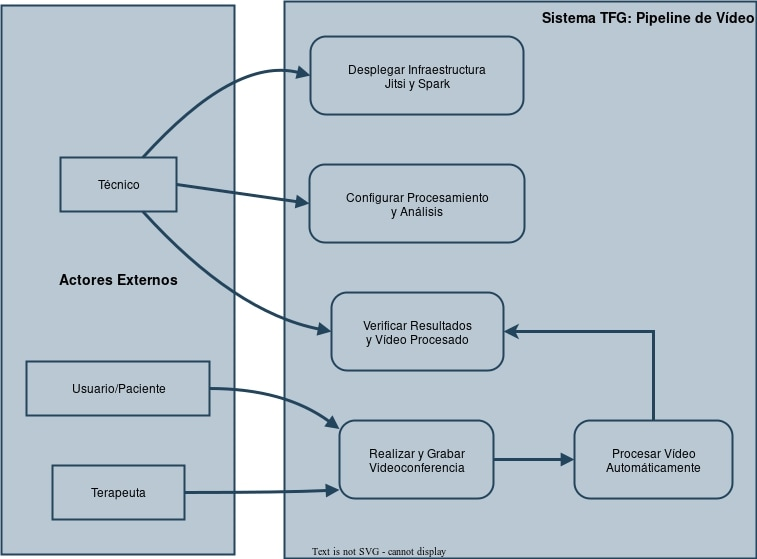
\includegraphics[width=0.8\textwidth]{img/Diagramacasodeuso.jpg}
    \caption{Diagrama de los principales casos de uso del sistema.}
    \label{fig:anexob_actores}
\end{figure}

\section{Catálogo de Requisitos Funcionales}
\label{sec:requisitos_funcionales}
A continuación, se detallan los requisitos funcionales del sistema, descritos como un flujo de trabajo lógico desde la perspectiva de los actores.

\begin{itemize}
	\item \textbf{RF.1: Realización de una Sesión de Telerehabilitación}
	\begin{itemize}
	    \item \textbf{RF.1.1:} El Paciente debe poder unirse a una sala de videoconferencia de Jitsi a través de un enlace web.
	    \item \textbf{RF.1.2:} El Terapeuta debe poder unirse a la misma sala de videoconferencia para dirigir la sesión.
	\end{itemize}
	
	\item \textbf{RF.2: Gestión de la Grabación de la Sesión}
	\begin{itemize}
	    \item \textbf{RF.2.1:} El Terapeuta debe disponer de un botón o función en la interfaz de Jitsi para iniciar la grabación de la sesión.
	    \item \textbf{RF.2.2:} Al iniciar la grabación, el sistema debe activar automáticamente el servicio Jibri, que se unirá a la llamada como un participante silencioso.
	    \item \textbf{RF.2.3:} El Terapeuta debe poder detener la grabación en cualquier momento.
        \item \textbf{RF.2.4:} Al detener la grabación, el sistema debe guardar la sesión completa como un único archivo de vídeo en formato MP4 en un directorio de entrada predefinido en el servidor.
	\end{itemize}
	
	\item \textbf{RF.3: Procesamiento Automático del Vídeo Grabado}
	\begin{itemize}
	    \item \textbf{RF.3.1:} El sistema debe detectar automáticamente cuándo un nuevo fichero MP4 ha sido depositado en el directorio de entrada.
	    \item \textbf{RF.3.2:} El sistema debe iniciar un proceso que tome el nuevo vídeo y lo envíe a través del pipeline de datos.
	    \item \textbf{RF.3.3:} El pipeline debe aplicar una transformación de vídeo predefinida (la prueba de concepto de inversión de color) a todos los fotogramas del vídeo.
	    \item \textbf{RF.3.4:} El sistema debe guardar el vídeo resultante de la transformación en un directorio de salida.
	\end{itemize}
	
	\item \textbf{RF.4: Gestión de Ficheros y Resultados}
	\begin{itemize}
	    \item \textbf{RF.4.1:} El Administrador del Sistema debe poder acceder al directorio de salida para verificar el vídeo procesado.
	    \item \textbf{RF.4.2:} Una vez que un vídeo original ha sido procesado con éxito, el sistema debe moverlo automáticamente a una carpeta de archivado para evitar que sea procesado de nuevo.
	\end{itemize}
\end{itemize}

\section{Casos de Uso}
A continuación, se describen los principales casos de uso desde la perspectiva del Administrador del Sistema.

\subsection{Caso de Uso 1: Desplegar la Infraestructura Completa}
\begin{itemize}
    \item \textbf{Actor:} Administrador del Sistema.
    \item \textbf{Descripción:} El administrador despliega todos los servicios de la arquitectura (Jitsi, Kafka, Spark, etc.) en un entorno limpio.
    \item \textbf{Precondiciones:} El sistema anfitrión (Debian 12) tiene Docker y Docker Compose instalados.
    \item \textbf{Flujo Principal:}
        \begin{enumerate}
            \item El administrador clona el repositorio del proyecto desde GitHub.
            \item El administrador configura los ficheros \texttt{.env} necesarios.
            \item El administrador ejecuta el comando \texttt{docker-compose up} principal.
            \item El sistema levanta todos los contenedores, crea las redes y los volúmenes necesarios.
        \end{enumerate}
    \item \textbf{Postcondiciones:} Todos los servicios están en ejecución y listos para operar.
\end{itemize}

\subsection{Caso de Uso 2: Ejecutar el Pipeline de Procesamiento de Vídeo}
\begin{itemize}
    \item \textbf{Actor:} Administrador del Sistema (o un proceso automatizado).
    \item \textbf{Descripción:} El administrador inicia el script que procesa un vídeo grabado previamente.
    \item \textbf{Precondiciones:} La infraestructura está desplegada y en ejecución. Existe al menos un archivo MP4 en el directorio de entrada.
    \item \textbf{Flujo Principal:}
        \begin{enumerate}
            \item El administrador ejecuta el script de procesamiento de vídeo.
            \item El script detecta el vídeo más antiguo en la carpeta de entrada.
            \item Los datos del vídeo se envían a través de Kafka y son procesados por Spark.
            \item Se genera un nuevo archivo de vídeo procesado en el directorio de salida.
            \item El archivo de vídeo original se mueve al directorio de archivado.
        \end{enumerate}
    \item \textbf{Postcondiciones:} El vídeo ha sido procesado y archivado. El sistema queda a la espera de nuevos vídeos.
\end{itemize}

\section{Especificación de requisitos}
En este apartado se van a mostrar, por una parte el diagrama de caso de uso, como se puede observar en las figuras  \ref{f:casoUso} y por otra, las tablas de casos de uso.


\begin{figure}[H]
 \centering
\subfloat{
    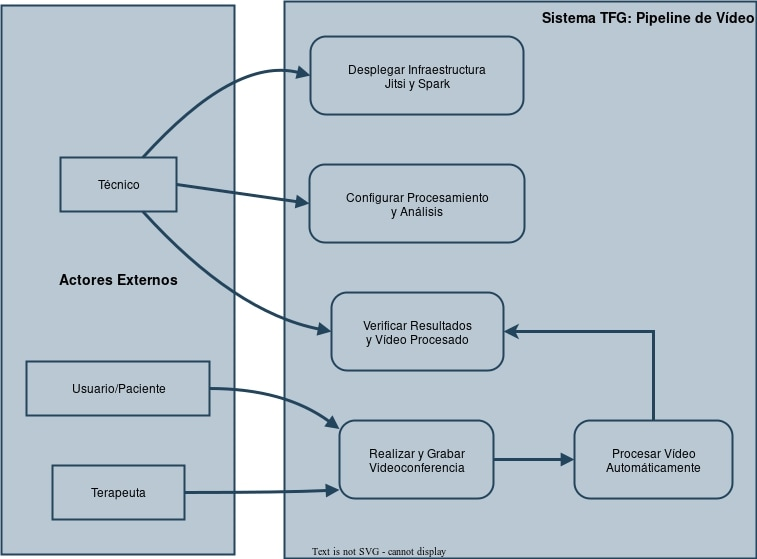
\includegraphics[width=\textwidth]{img/Diagramacasodeuso.jpg}}
 \caption{Diagrama de casos de uso.}
 \label{f:casoUso}
\end{figure}


% --- CASO DE USO 1 ---
\begin{table}[H]
    \centering
    \caption{Caso de uso 1: Desplegar la Infraestructura Completa.}
    \label{tab:uc1}
    \begin{tabular}{|p{3cm}|p{0.75cm}|p{8.5cm}|}
        \hline
        \textbf{Descripción} & \multicolumn{2}{p{9.25cm}|}{Permite al Administrador del Sistema desplegar todos los servicios de la arquitectura de forma orquestada.} \\
        \hline
        \multirow{3}{3cm}{\textbf{Requisitos}} & \multicolumn{2}{p{9.25cm}|}{RF.1.1} \\ \cline{2-3}
         & \multicolumn{2}{p{9.25cm}|}{RF.1.2} \\ \cline{2-3}
         & \multicolumn{2}{p{9.25cm}|}{RF.1.3} \\
        \hline
        \textbf{Precondiciones} & \multicolumn{2}{p{9.25cm}|}{El sistema anfitrión (Debian 12) tiene Docker y Docker Compose instalados y funcionando correctamente.} \\
        \hline
        \multirow{4}{3cm}{\textbf{Secuencia Normal}} & \textbf{Paso} & \textbf{Acción} \\ \cline{2-3}
         & 1 & El Administrador clona el repositorio del proyecto desde GitHub. \\ \cline{2-3}
         & 2 & El Administrador configura los ficheros de entorno (\texttt{.env}) necesarios. \\ \cline{2-3}
         & 3 & El Administrador ejecuta el comando \texttt{docker-compose up} desde la raíz del proyecto. \\ \cline{2-3}
         & 4 & El sistema levanta todos los contenedores, crea las redes y los volúmenes necesarios. \\
        \hline
        \textbf{Postcondiciones} & \multicolumn{2}{p{9.25cm}|}{Todos los servicios de la infraestructura (Jitsi, Kafka, Spark) están en ejecución y listos para operar.} \\
        \hline
        \textbf{Excepciones} & \multicolumn{2}{p{9.25cm}|}{El host no tiene conexión a internet, lo que impide la descarga de las imágenes Docker desde los registros públicos.} \\
        \hline
        \textbf{Importancia} & \multicolumn{2}{p{9.25cm}|}{Alta} \\
        \hline
        \textbf{Urgencia} & \multicolumn{2}{p{9.25cm}|}{Alta} \\
        \hline
    \end{tabular}
\end{table}

% --- CASO DE USO 2 ---
\begin{table}[H]
    \centering
    \caption{Caso de uso 2: Ejecutar el Pipeline de Procesamiento de Vídeo.}
    \label{tab:uc2}
    \begin{tabular}{|p{3cm}|p{0.75cm}|p{8.5cm}|}
        \hline
        \textbf{Descripción} & \multicolumn{2}{p{9.25cm}|}{Permite procesar un vídeo grabado en una sesión de Jitsi para obtener un resultado analizado.} \\
        \hline
        \multirow{4}{3cm}{\textbf{Requisitos}} & \multicolumn{2}{p{9.25cm}|}{RF.2.1, RF.2.2, RF.3.1, RF.3.2, RF.3.3, RF.4.1, RF.4.2, RF.4.3} \\
        \hline
        \textbf{Precondiciones} & \multicolumn{2}{p{9.25cm}|}{La infraestructura está desplegada y en ejecución. Se ha realizado una sesión de telerehabilitación y el archivo MP4 resultante se encuentra en el directorio de entrada.} \\
        \hline
        \multirow{4}{3cm}{\textbf{Secuencia Normal}} & \textbf{Paso} & \textbf{Acción} \\ \cline{2-3}
         & 1 & El Terapeuta inicia y finaliza la grabación de una sesión en Jitsi. Jibri guarda el fichero MP4. \\ \cline{2-3}
         & 2 & El Administrador (o un proceso automatizado) ejecuta el script de procesamiento. \\ \cline{2-3}
         & 3 & El script detecta el vídeo, lo procesa a través del pipeline Kafka/Spark y guarda el resultado. \\ \cline{2-3}
         & 4 & El script archiva el vídeo original para evitar su reprocesamiento. \\
        \hline
        \textbf{Postcondiciones} & \multicolumn{2}{p{9.25cm}|}{El vídeo ha sido procesado y el resultado se encuentra en el directorio de salida. El vídeo original ha sido archivado.} \\
        \hline
        \textbf{Excepciones} & \multicolumn{2}{p{9.25cm}|}{No hay vídeos nuevos en el directorio de entrada; el script finaliza sin realizar ninguna acción.} \\
        \hline
        \textbf{Importancia} & \multicolumn{2}{p{9.25cm}|}{Alta} \\
        \hline
        \textbf{Urgencia} & \multicolumn{2}{p{9.25cm}|}{Alta} \\
        \hline
    \end{tabular}
\end{table}
\apendice{Especificación de Diseño}
\label{apendice:diseno}

\section{Introducción}
La fase de diseño permite planificar un proyecto para su correcta implementación, desarrollo y evolución. En este anexo se exponen los diferentes diseños que se han llevado a cabo para obtener una solución robusta y escalable a los problemas planteados. Se detallará el diseño de los datos que maneja el sistema, el diseño arquitectónico de alto nivel, y el diseño procedimental que describe el flujo de trabajo del pipeline.

\section{Diseño de Datos}
\label{sec:diseno_datos}
El diseño de datos se centra en la estructura y el formato de la información que fluye a través del sistema. Aunque el dato principal es el vídeo, su tratamiento y los metadatos asociados son clave.

\subsection{Objeto de Datos Principal: Vídeo de Sesión}
El dato principal que se procesa es el archivo de vídeo generado por Jibri. Este es un fichero en formato \textbf{MP4}, que contiene un \textit{stream} de vídeo codificado (normalmente con el \textit{códec} H.264) y un \textit{stream} de audio.

\subsection{Formato de Salida del Procesamiento}
Una de las tareas de la fase final del proyecto es definir el formato de salida que generará el \textit{script} de Spark. Se ha establecido que el resultado será un nuevo fichero de vídeo también en formato MP4. Para una futura evolución del proyecto donde se extraigan características específicas, se podría definir un formato de datos estructurado (como JSON o Avro) que contenga metadatos como:
\begin{itemize}
    \item \texttt{id\_sesion}: Identificador único de la sesión grabada.
    \item \texttt{timestamp}: Marca de tiempo del procesamiento.
    \item \texttt{algoritmo\_aplicado}: Nombre de la transformación realizada (ej. "inversion-color").
    \item \texttt{ruta\_video\_procesado}: Ruta al fichero de vídeo resultante.
    \item \texttt{métricas}: Un objeto que podría contener métricas de análisis (ej. número de objetos detectados, nivel de movimiento, etc.).
\end{itemize}

\section{Diseño Arquitectónico}
\label{sec:diseno_arquitectonico}
El diseño arquitectónico define la estructura de alto nivel del sistema, sus componentes principales y las interacciones entre ellos.

\subsection{Diagrama de Arquitectura General del Sistema}
La arquitectura general se ha diseñado como un sistema distribuido basado en micro-servicios, donde cada componente tiene una responsabilidad única. La Figura \ref{fig:arquitectura_general} ofrece una visión completa de la solución, desde la captura de vídeo hasta el procesamiento final.

\begin{figure}[H]
    \centering
    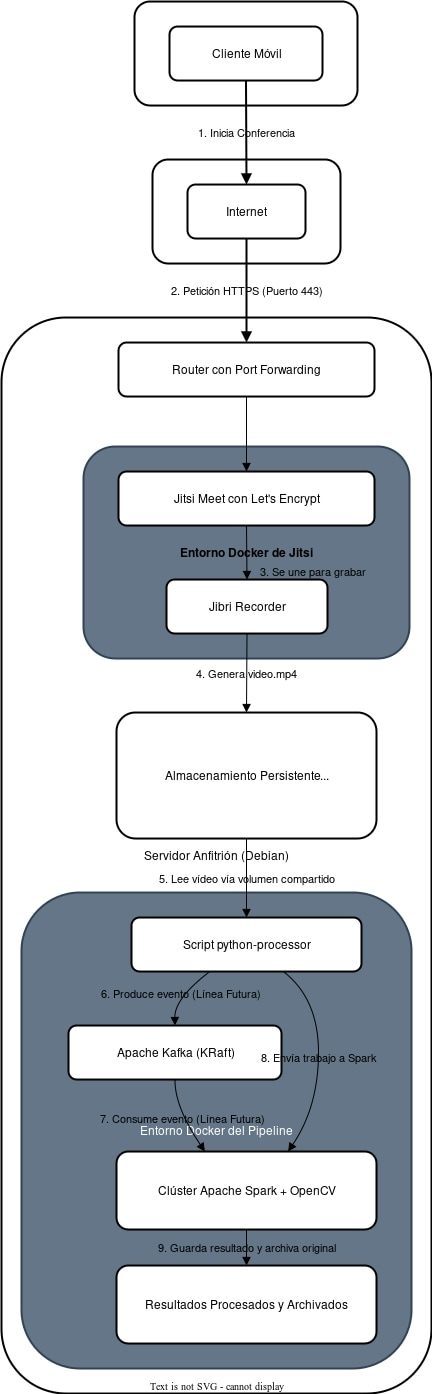
\includegraphics[height=\textheight]{img/arquitectura-general.jpg}
    \caption{Diagrama de la arquitectura general del sistema.}
    \label{fig:arquitectura_general}
\end{figure}

Como se puede observar, el sistema se divide en tres grandes bloques: el subsistema de captura de vídeo (basado en Jitsi), el pipeline de datos (orquestado con Docker Compose y centrado en Kafka y Spark), y el almacenamiento persistente.

\subsection{Diagrama de la Arquitectura de Red para Jitsi}
El despliegue de Jitsi para que fuera accesible desde el exterior de forma segura fue uno de los principales desafíos técnicos. La solución final, representada en la Figura \ref{fig:arquitectura_red}, se basa en una configuración de red que incluye un servicio de DNS dinámico, redirección de puertos y la generación de certificados SSL/TLS con Let's Encrypt.

\begin{figure}[H]
    \centering
    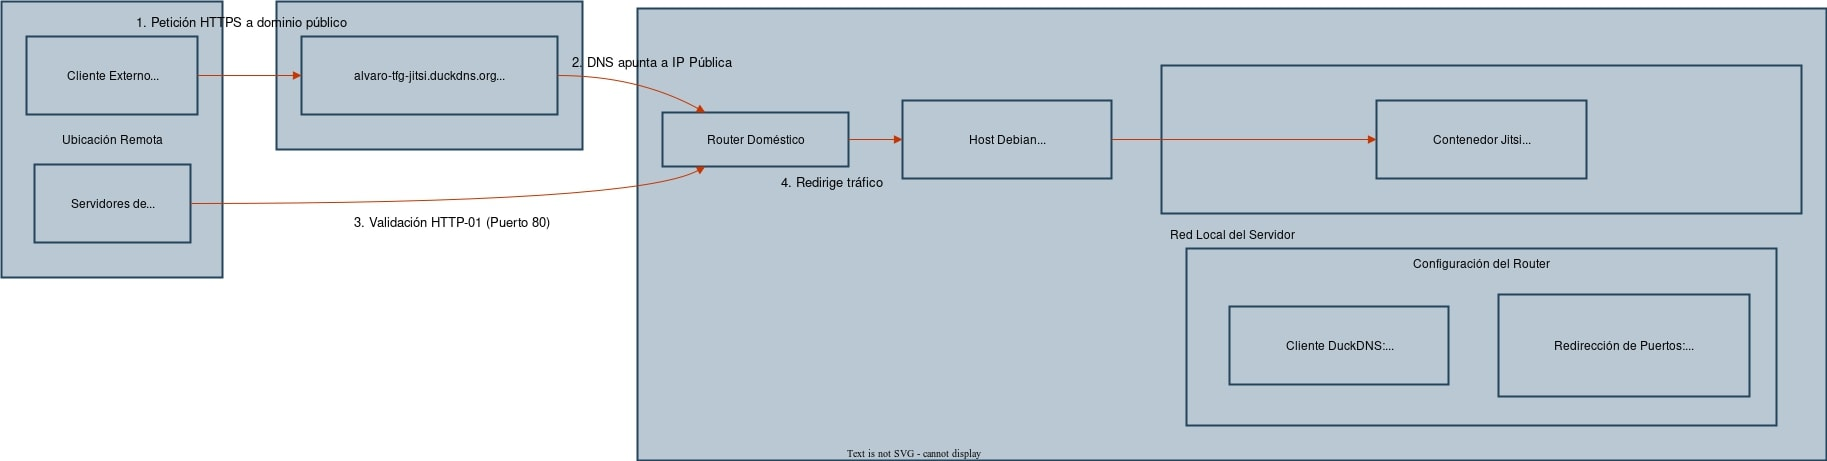
\includegraphics[width=1\textwidth]{img/ArquitecturadeRedparaelDesplieguedeJitsi.jpg}
    \caption{Arquitectura de red para el despliegue seguro de Jitsi.}
    \label{fig:arquitectura_red}
\end{figure}

\section{Diseño Procedimental}
\label{sec:diseno_procedimental}
El diseño procedimental describe la secuencia de pasos y el flujo de control del sistema.

\subsection{Flujo de Datos del Pipeline de Procesamiento}
El núcleo de la lógica de negocio reside en el pipeline implementado dentro del directorio \texttt{/src}. El flujo de datos (ver Figura \ref{fig:flujo_pipeline}) describe la interacción entre el \textit{script} de Python, Kafka y Spark para procesar los vídeos de forma automatizada.

\begin{figure}[H]
    \centering
    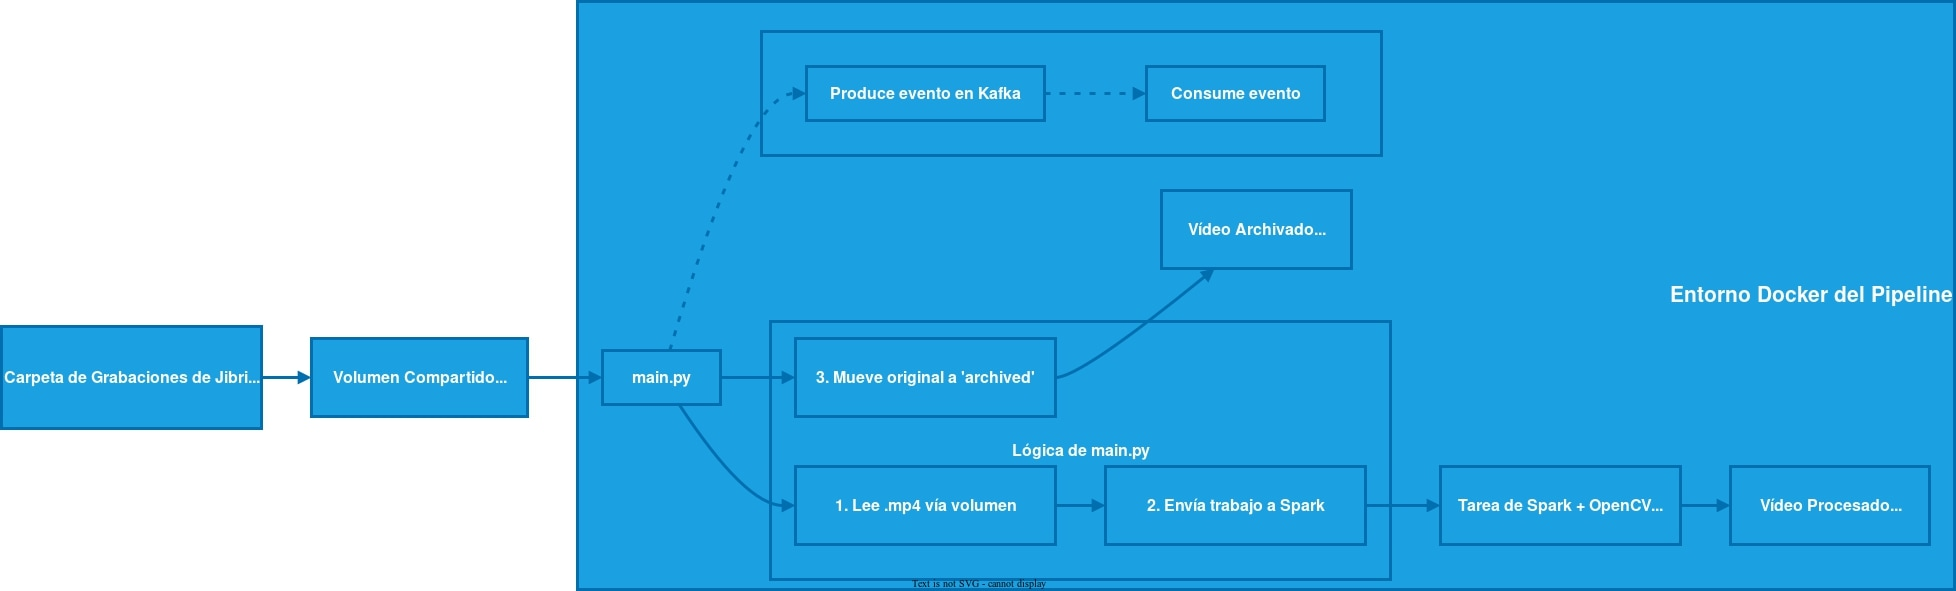
\includegraphics[width=\textwidth]{img/FlujodeDatosdelPipelinedeProcesamiento.jpg}
    \caption{Diagrama de flujo de datos del pipeline de procesamiento.}
    \label{fig:flujo_pipeline}
\end{figure}

El proceso comienza cuando el \textit{script} principal detecta un nuevo archivo MP4. Este archivo es enviado como un mensaje a Kafka. Un consumidor de Spark recibe el mensaje, ejecuta la lógica de procesamiento y guarda el resultado, archivando finalmente el vídeo original.

\subsection{Funcionamiento Interno de la Grabación de Jibri}
Para comprender cómo se genera la fuente de datos, es útil visualizar el funcionamiento interno de Jibri (Figura \ref{fig:flujo_jibri}). Jibri lanza una instancia de un navegador en modo \textit{headless} que se une a la conferencia, renderiza la vista compuesta y utiliza FFmpeg para capturar esta salida y codificarla en un archivo MP4.

\begin{figure}[H]
    \centering
    \includegraphics[width=0.8\textwidth]{img/ProcesoInternodeGrabacióndeJibri..jpg}
    \caption{Diagrama conceptual del proceso de grabación de Jibri.}
    \label{fig:flujo_jibri}
\end{figure}

\subsection{Casos de Uso del Sistema}
Finalmente, el diagrama de casos de uso (Figura \ref{fig:casos_uso}) muestra la interacción de los diferentes actores (Técnico, Usuario, Terapeuta) con las funcionalidades principales del sistema.

\begin{figure}[H]
    \centering
    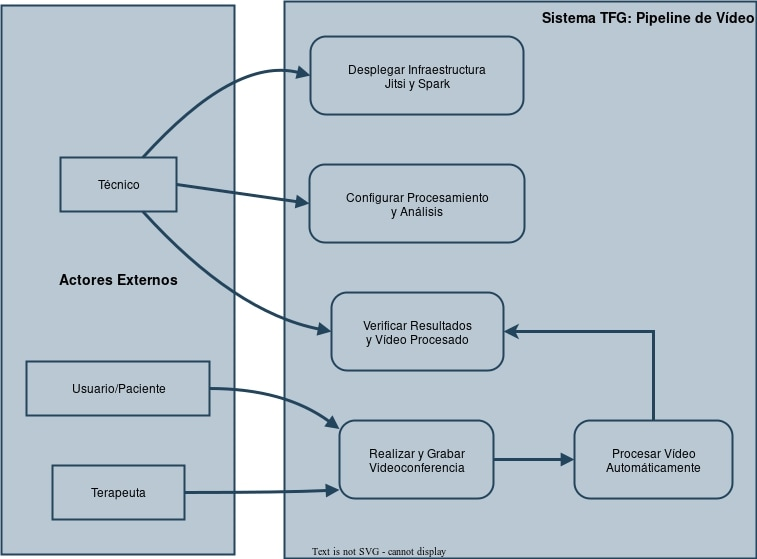
\includegraphics[width=0.7\textwidth]{img/Diagramacasodeuso.jpg}
    \caption{Diagrama de los principales casos de uso del sistema.}
    \label{fig:casos_uso}
\end{figure}

\subsection{Flujo Detallado de Transformación en Spark}
Para comprender en profundidad cómo se procesan los datos una vez que llegan al consumidor de Spark, la Figura \ref{fig:flujo_transformacion_spark} detalla el flujo de transformación de paquetes que se ejecuta dentro del script de PySpark.

\begin{figure}[H]
    \centering
    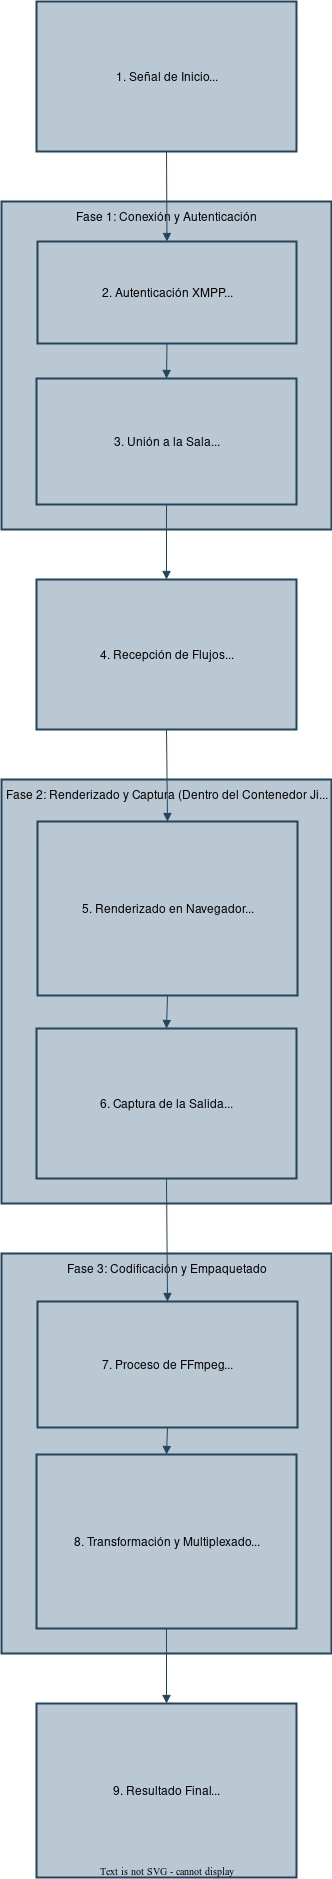
\includegraphics[height=\textheight]{img/FlujoDetalladodeTransformaciondePaquetes.jpg}
    \caption{Diagrama de flujo detallado del procesamiento de vídeo en Spark.}
    \label{fig:flujo_transformacion_spark}
\end{figure}

El proceso procedimental es el siguiente:
\begin{enumerate}
    \item El consumidor Spark recibe un mensaje desde el \textit{topic} de Kafka. Este mensaje contiene los datos o la referencia al vídeo a procesar.
    \item Los datos son pasados a una función de procesamiento definida por el usuario.
    \item Dentro de esta función, se utiliza la librería OpenCV para abrir el fichero de vídeo y comenzar a leerlo fotograma a fotograma.
    \item Se itera sobre cada \textit{frame}: se aplica la transformación de vídeo correspondiente (en la prueba de concepto, una inversión de color) y el \textit{frame} modificado se escribe en un nuevo fichero de vídeo de salida.
    \item Una vez procesados todos los \textit{frames}, se cierra el flujo de escritura, finalizando la creación del vídeo procesado.
\end{enumerate}
Este diseño modular permite que la lógica de transformación (paso 4) pueda ser fácilmente modificada o extendida en el futuro para aplicar análisis más complejos.

Para poder ver correctamente los diagramas debido a su tamaño se recomienda descargarlos de la documentación.
\apendice{Documentación Técnica de Programación}
\label{apendice:doc_tecnica}


\section{Introducción}
Este anexo está dirigido a un perfil técnico (un futuro desarrollador o evaluador del proyecto) y tiene como objetivo detallar la estructura del código, la arquitectura de los componentes de software, las decisiones de diseño y el proceso completo de compilación y despliegue del sistema. La finalidad es que cualquier persona con los conocimientos técnicos adecuados pueda comprender, replicar y extender el trabajo realizado.

\section{Estructura de Directorios del Repositorio}
\label{sec:doc_tecnica_directorios}
La organización del repositorio en GitHub ha sido una pieza clave para mantener el proyecto ordenado y comprensible. A continuación, se expone la estructura de directorios que cuelgan desde la raíz del proyecto.

\subsection{Directorio de Documentación (`/docs`)}
La carpeta \texttt{/docs} contiene toda la documentación del proyecto, principalmente la memoria del TFG y sus recursos asociados. Su estructura es la siguiente:

\dirtree{%
.1 /docs.
.2 /diagrams.
.2 /images.
.2 /tex.
.2 memoria.tex.
.2 anexos.tex.
.2 bibliografia.bib.
}

\begin{itemize}
    \item \texttt{/diagrams}: Almacena los ficheros fuente de los diagramas del proyecto (por ejemplo, los archivos de \textit{Diagrams.net}).
    \item \texttt{/images} (o \texttt{/img}): Contiene los ficheros de imagen (PNG, JPG) que se insertan en la memoria, como capturas de pantalla o los diagramas exportados.
    \item \texttt{/tex}: Contiene los ficheros \texttt{.tex} individuales para cada capítulo y apéndice de la memoria, permitiendo una organización modular del documento.
    \item \texttt{memoria.tex} y \texttt{anexos.tex}: Son los ficheros principales de \LaTeX{} que estructuran y compilan el documento final.
    \item \texttt{bibliografia.bib}: Fichero de BibTeX que contiene todas las referencias bibliográficas citadas.
\end{itemize}

\subsection{Directorio de Configuración del Despliegue}
Esta carpeta contiene los ficheros de configuración validados y necesarios para desplegar los sistemas de terceros, principalmente Jitsi. No contiene una instancia de Jitsi, sino las plantillas para configurarla a partir del repositorio oficial.

\dirtree{%
.1 /configuracion\_despliegue.
.2 /jitsi.
.3 .gitkeep.
.3 README.md.
.3 docker-compose.yml.
.3 env.example.
.3 gen-passwords.sh.
.3 jibri.yml.
}
Un desarrollador que desee replicar el entorno debe clonar el repositorio oficial de \texttt{docker-jitsi-meet} y utilizar los ficheros de esta carpeta como base para su configuración.

\subsection{Directorio de Código Fuente (`/src`)}
La carpeta \texttt{/src} es el corazón del proyecto. Contiene todo el código fuente de la aplicación de procesamiento y su fichero de orquestación con Docker Compose.

\dirtree{%
.1 /src.
.2 /data.
.3 /processed.
.4 .gitkeep.
.3 .gitkeep.
.2 /dockers.
.3 /python\_processor.
.4 main.py.
.4 requirements.txt.
.4 Dockerfile.
.2 docker-compose.yml.
}

\begin{itemize}
    \item \texttt{docker-compose.yml}: Es el fichero de orquestación que define y levanta los servicios del pipeline de procesamiento de datos: Kafka, Spark (master y worker) y el procesador Python.
    \item \texttt{/dockers/python\_processor}: Contiene la lógica de la aplicación principal.
        \begin{itemize}
            \item \texttt{Dockerfile}: Instrucciones para construir la imagen Docker del servicio.
            \item \texttt{requirements.txt}: Lista de las librerías de Python necesarias para el proyecto.
            \item \texttt{main.py}: El script principal que contiene la lógica para detectar, procesar y archivar los vídeos.
        \end{itemize}
    \item \texttt{/data}: Actúa como punto de montaje principal para los datos de vídeo. Los vídeos grabados por Jibri se mapean a este directorio para que el pipeline los pueda procesar. Contiene a su vez las subcarpetas \texttt{/processed} y \texttt{/archived} para almacenar los resultados y los ficheros originales, respectivamente.
\end{itemize}

\section{Manual del Programador (Arquitectura del Software)}

\subsection{Arquitectura Modular}
El sistema se ha diseñado siguiendo un enfoque modular, separando claramente dos responsabilidades principales:
\begin{itemize}
    \item \textbf{Sistema de Captura (Jitsi):} Se encarga exclusivamente de la captura y grabación de las sesiones de vídeo, generando los archivos MP4.
    \item \textbf{Pipeline de Procesamiento (Kafka/Spark):} Es un sistema independiente que se encarga de consumir y procesar dichos archivos.
\end{itemize}
Esta separación facilita el desarrollo, las pruebas y la escalabilidad, ya que cada componente puede ser modificado o sustituido sin afectar al otro.

\subsection{Arquitectura del Pipeline de Procesamiento}
La Figura \ref{fig:flujo_pipeline} (incluida en el Apéndice de Diseño) ilustra la interacción entre los servicios definidos en el fichero \texttt{docker-compose.yml} de la carpeta \texttt{/src}.
\begin{itemize}
    \item \textbf{Kafka:} Actúa como \textit{broker} de mensajería para desacoplar el sistema. Funciona en modo KRaft, sin dependencia de Zookeeper.
    \item \textbf{Spark (Master/Worker):} Conforman el clúster de cómputo donde se ejecutan las tareas de procesamiento de vídeo.
    \item \textbf{python-processor:} Es el servicio principal que contiene la lógica de negocio. Orquesta todo el flujo: detecta los vídeos, los envía a Kafka, y consume los resultados de Spark.
\end{itemize}

\begin{figure}[H]
    \centering
    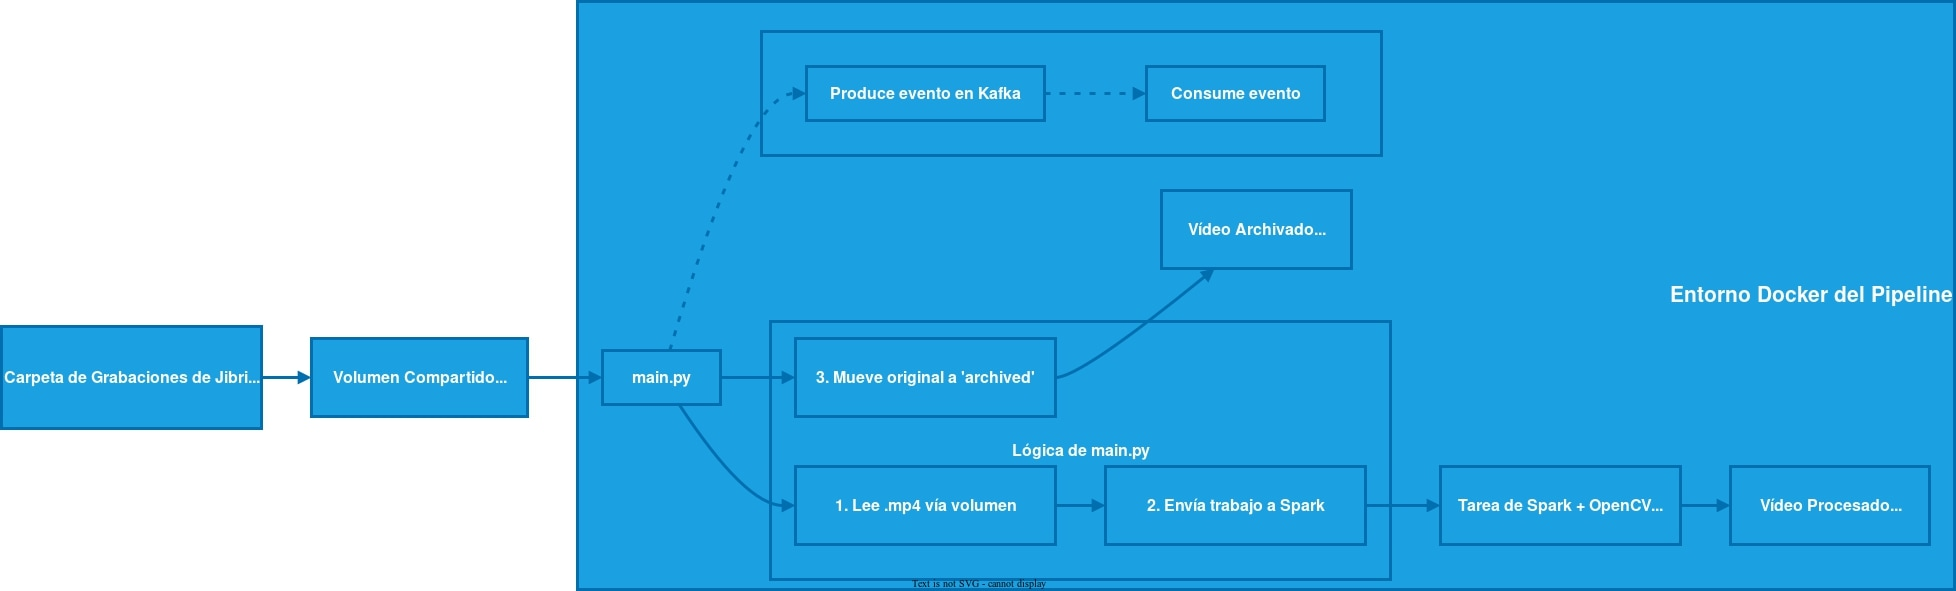
\includegraphics[width=\textwidth]{img/FlujodeDatosdelPipelinedeProcesamiento.jpg}
    \caption{Diagrama de flujo de datos del pipeline de procesamiento implementado en la carpeta /src.}
    \label{fig:apendice_d_flujo_pipeline}
\end{figure}

\subsection{Descripción del Script \texttt{main.py}}
El script \texttt{main.py} es el cerebro de la aplicación. Su lógica principal es la siguiente:
\begin{enumerate}
    \item Establece una conexión con la sesión de Spark para poder enviar trabajos de procesamiento.
    \item Entra en un bucle que busca el vídeo más antiguo en la carpeta de entrada (\texttt{/data}), ignorando explícitamente los subdirectorios \texttt{/processed} y \texttt{/archived}.
    \item Si encuentra un vídeo, lo envía a un \textit{topic} de Kafka y espera el resultado del procesamiento.
    \item Una vez procesado, guarda el vídeo resultante y archiva el original.
\end{enumerate}

\begin{figure}[H]
    \centering
    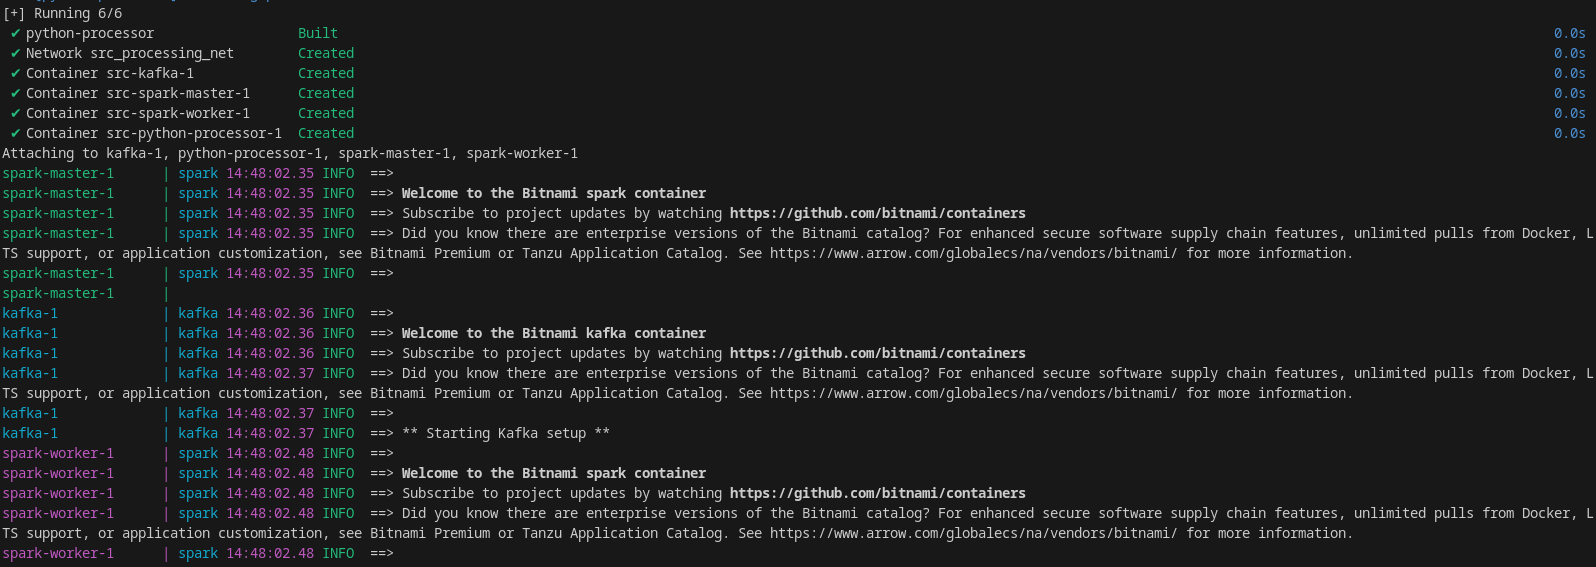
\includegraphics[width=\textwidth]{img/montarsparkkafka.png}
    \caption{Salida de la terminal mostrando el despliegue de los servicios del pipeline (Kafka, Spark, etc.) con Docker Compose.}
    \label{fig:apendice_d_compose_up}
\end{figure}

\subsection{Construcción de la Imagen Docker (Dockerfile)}
El \texttt{Dockerfile} del servicio \texttt{python-processor} define los pasos para construir su imagen. Las decisiones clave fueron:
\begin{itemize}
    \item Usar una imagen base oficial de Python (\texttt{python:3.9-slim}) por ser ligera y estable.
    \item Instalar las dependencias de sistema necesarias, como Java, que es un requisito para la comunicación con Spark.
    \item Instalar las librerías de Python especificadas en el fichero \texttt{requirements.txt}, \\ fijando las versiones para garantizar la reproducibilidad y evitar conflictos (como el surgido con NumPy).
\end{itemize}

\section{Compilación, Instalación y Ejecución del Proyecto}

\subsection{Configuración del Entorno Anfitrión}
Los requisitos detallados del sistema anfitrión se encuentran en el Apéndice E. Los puntos clave son el uso de Debian como sistema operativo, la instalación de Docker y Docker Compose, y la instalación del módulo del kernel \texttt{v4l2loopback-dkms} para el correcto funcionamiento de Jibri.

\subsection{La Crónica del Despliegue de Jitsi}
El despliegue de Jitsi fue uno de los mayores desafíos de ingeniería de este proyecto. El proceso de depuración se puede resumir en los siguientes hitos:
\begin{enumerate}
    \item \textbf{Fracaso en Windows/WSL2:} El intento inicial de despliegue en este entorno falló debido a problemas insuperables de permisos de ficheros y autenticación de los servicios.
    \item \textbf{Pivote a Debian:} Se tomó la decisión estratégica de migrar a un entorno Linux nativo, lo que solucionó los problemas de base.
    \item \textbf{Depuración de la Conexión:} Se resolvieron sucesivamente problemas de conexión WSS, errores de montaje del fichero \texttt{custom.config.js} y fallos de autenticación de usuarios invitados en Prosody.
    \item \textbf{Implementación de HTTPS:} Se descartó el uso de certificados autofirmados por problemas de confianza y se implementó una solución robusta con \textbf{Let's Encrypt}, para lo cual fue necesario configurar un dominio público con DuckDNS y re-dirección de puertos.
    \item \textbf{Diagnóstico del "Vídeo en Negro":} El problema final de la falta de vídeo en las grabaciones de Jibri se diagnosticó como una necesidad de permisos elevados, solucionándose al añadir la directiva \texttt{privileged: true} al servicio.
\end{enumerate}

\begin{figure}[H]
    \centering
    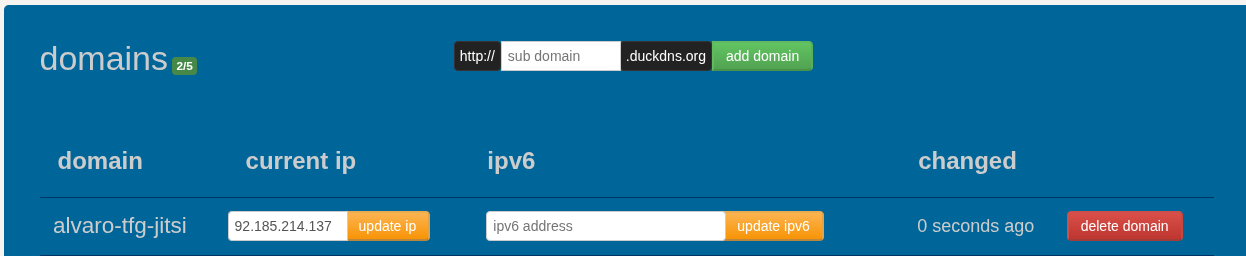
\includegraphics[width=0.9\textwidth]{img/duckdns.png}
    \caption{Configuración del dominio público en el servicio de DNS Dinámico DuckDNS.}
    \label{fig:apendice_d_duckdns}
\end{figure}

\begin{figure}[H]
    \centering
    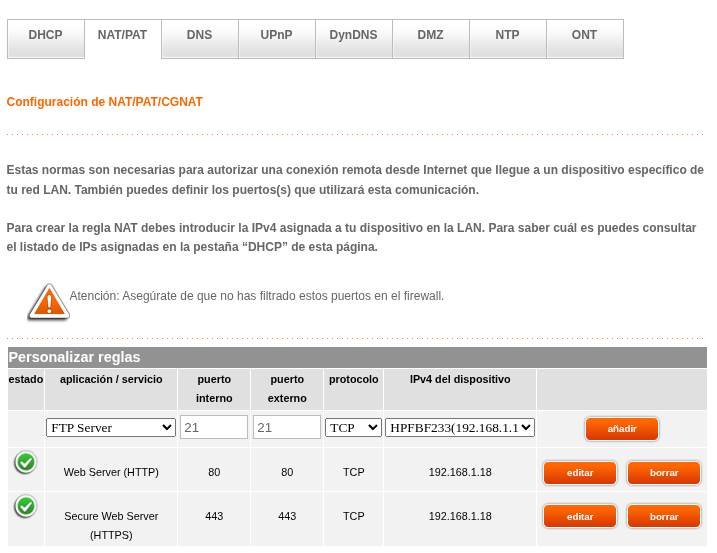
\includegraphics[width=0.9\textwidth]{img/routerconfig.png}
    \caption{Configuración de la redirección de puertos en el router para permitir el acceso externo a Jitsi.}
    \label{fig:apendice_d_router}
\end{figure}

\begin{figure}[H]
    \centering
    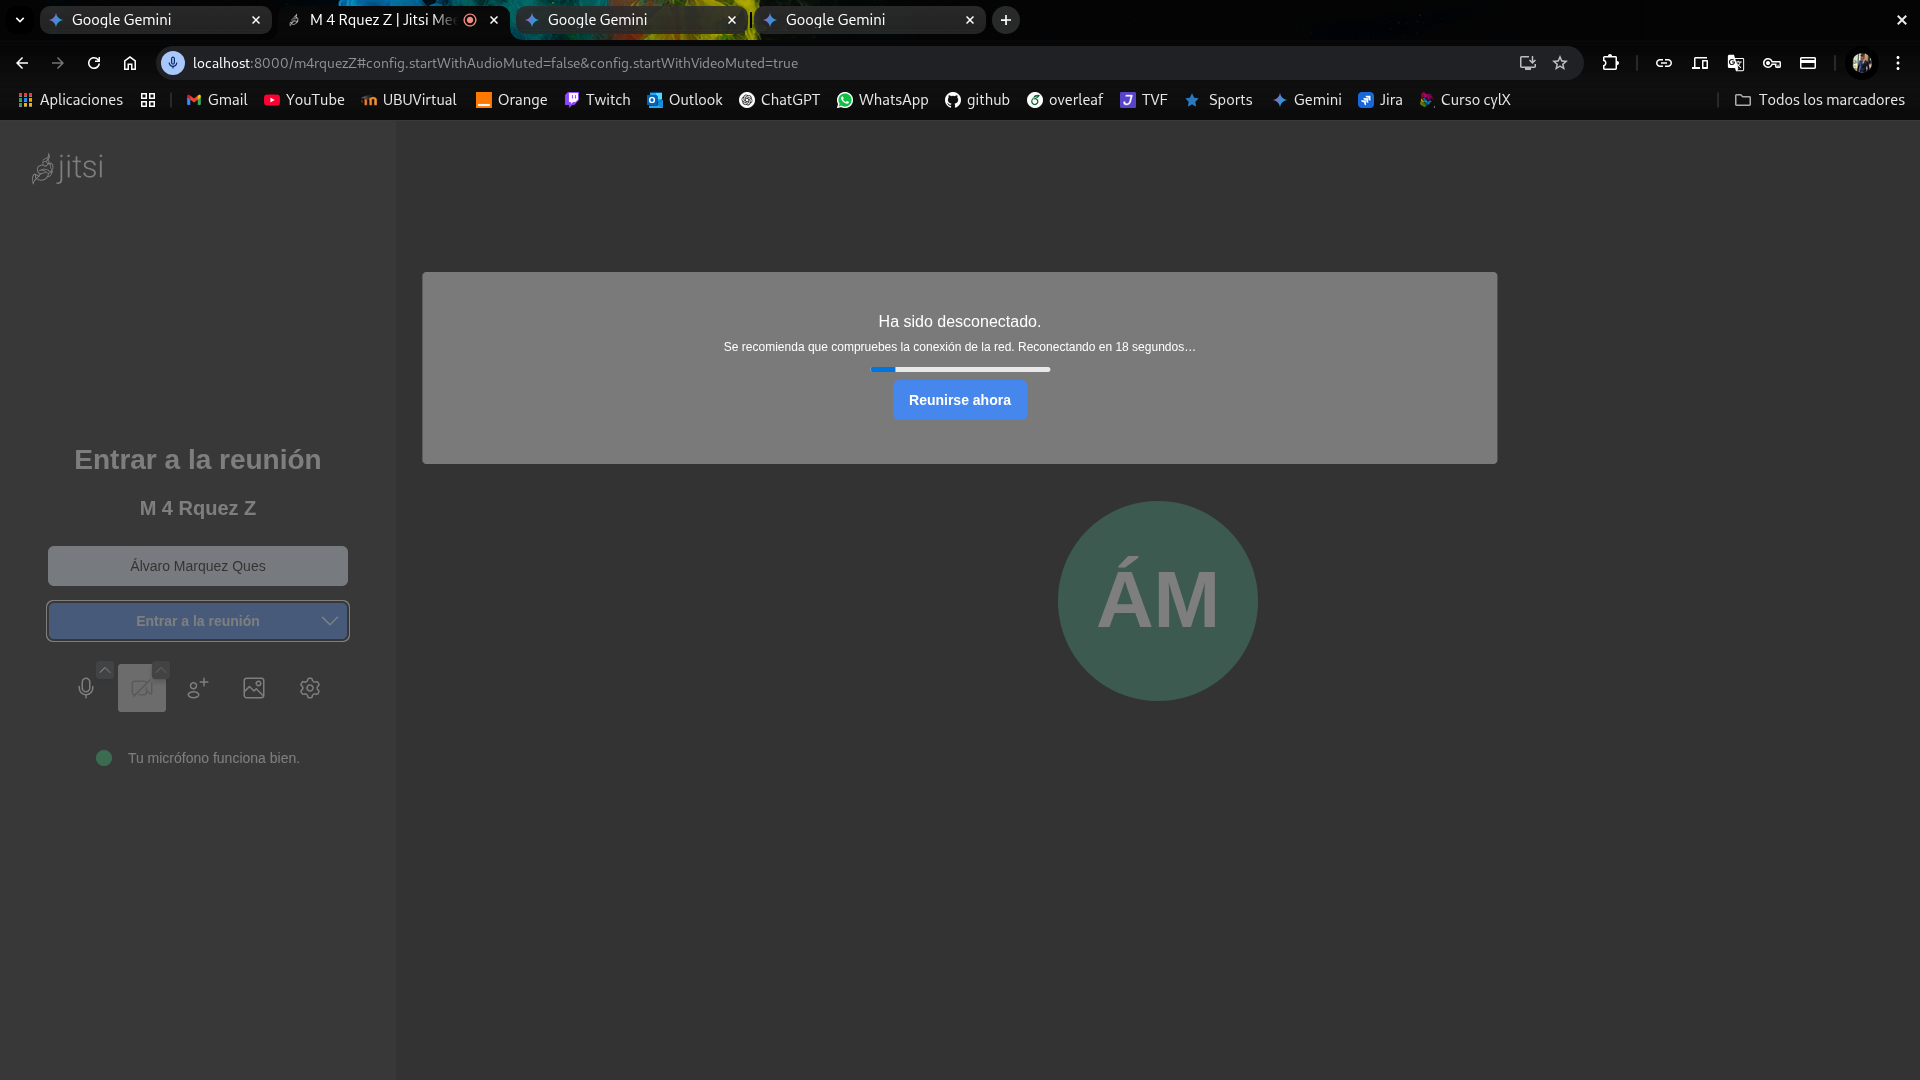
\includegraphics[width=0.7\textwidth]{img/errorconexion.png}
    \caption{Error de conexión encontrado durante la depuración de Jitsi en Debian.}
    \label{fig:apendice_d_error_conexion}
\end{figure}

\subsection{Despliegue del Pipeline de Procesamiento}
El despliegue de la pila de Kafka y Spark es un proceso automatizado. Al ejecutar \texttt{docker compose up} en el directorio \texttt{/src}, todos los servicios se inician en el orden correcto. La conexión con Jitsi se realiza a través del volumen Docker compartido que mapea la carpeta de grabaciones de Jibri al directorio de entrada del pipeline.

\begin{figure}[H]
    \centering
    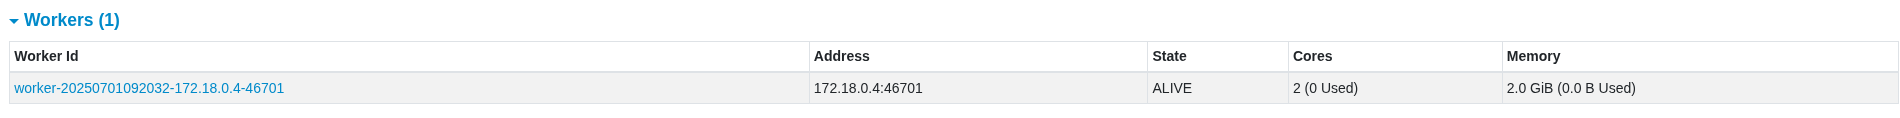
\includegraphics[width=0.9\textwidth]{img/workerpy.png}
    \caption{Captura de servicio \textit{worker} levantado y corriendo.}
    \label{fig:worker_py}
\end{figure}

\section{Pruebas del Sistema}

\subsection{Pruebas de Integración}
Se ha probado el flujo completo de extremo a extremo:
\begin{enumerate}
    \item Se inicia una conferencia en Jitsi y se graba.
    \item Se verifica que Jibri genera y guarda correctamente el archivo MP4.
    \item Se ejecuta el pipeline de procesamiento.
    \item Se comprueba en los \textit{logs} que el \textit{script} detecta el vídeo, lo procesa y lo archiva.
    \item Se verifica la existencia y el contenido del vídeo procesado en la carpeta de salida.
\end{enumerate}
Estas pruebas han validado que todos los componentes se comunican correctamente entre sí.

\subsection{Pruebas Funcionales (Prueba de Concepto)}
Para demostrar la funcionalidad del procesamiento, se ha implementado un algoritmo simple que invierte los colores de cada fotograma. La Figura \ref{fig:prueba_funcional} muestra una comparación entre un fotograma del vídeo original y el mismo fotograma del vídeo procesado, donde se puede apreciar visualmente el éxito de la transformación aplicada.

\begin{figure}[H]
    \centering
    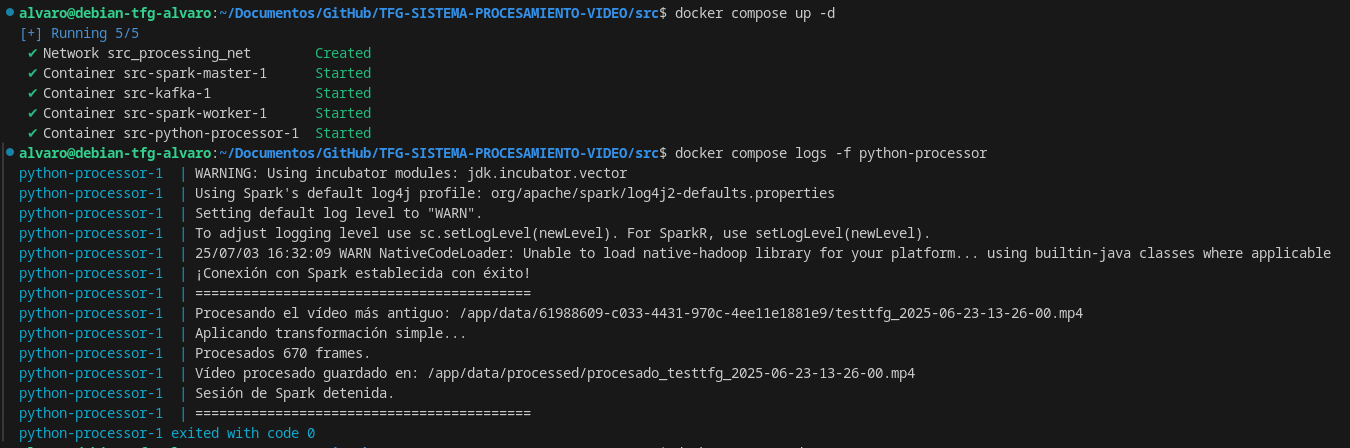
\includegraphics[width=\textwidth]{img/logsfinalpy.png}
    \caption{Logs del contenedor \texttt{python-processor} que muestran la ejecución exitosa del pipeline completo.}
    \label{fig:apendice_d_logs_finales}
\end{figure}
\begin{figure}[H]
    \centering
    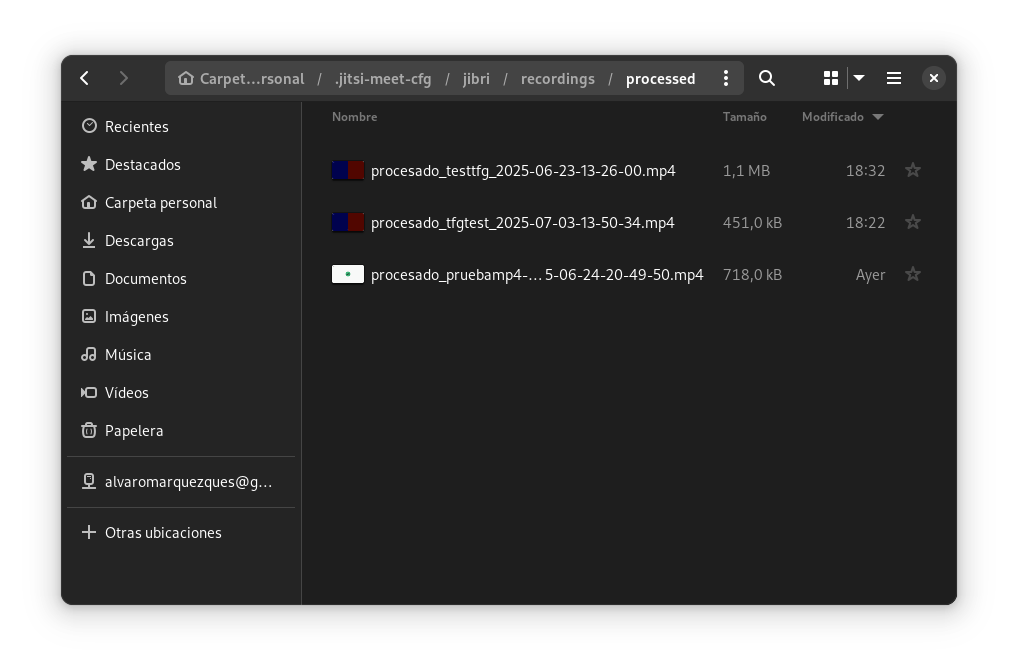
\includegraphics[width=1\textwidth]{img/carpetaprocessed.png}
    \caption{Directorio de salida con el fichero de vídeo ya procesado.}
    \label{fig:apendice_d_carpeta_procesado}
\end{figure}
\begin{figure}[H]
    \centering
    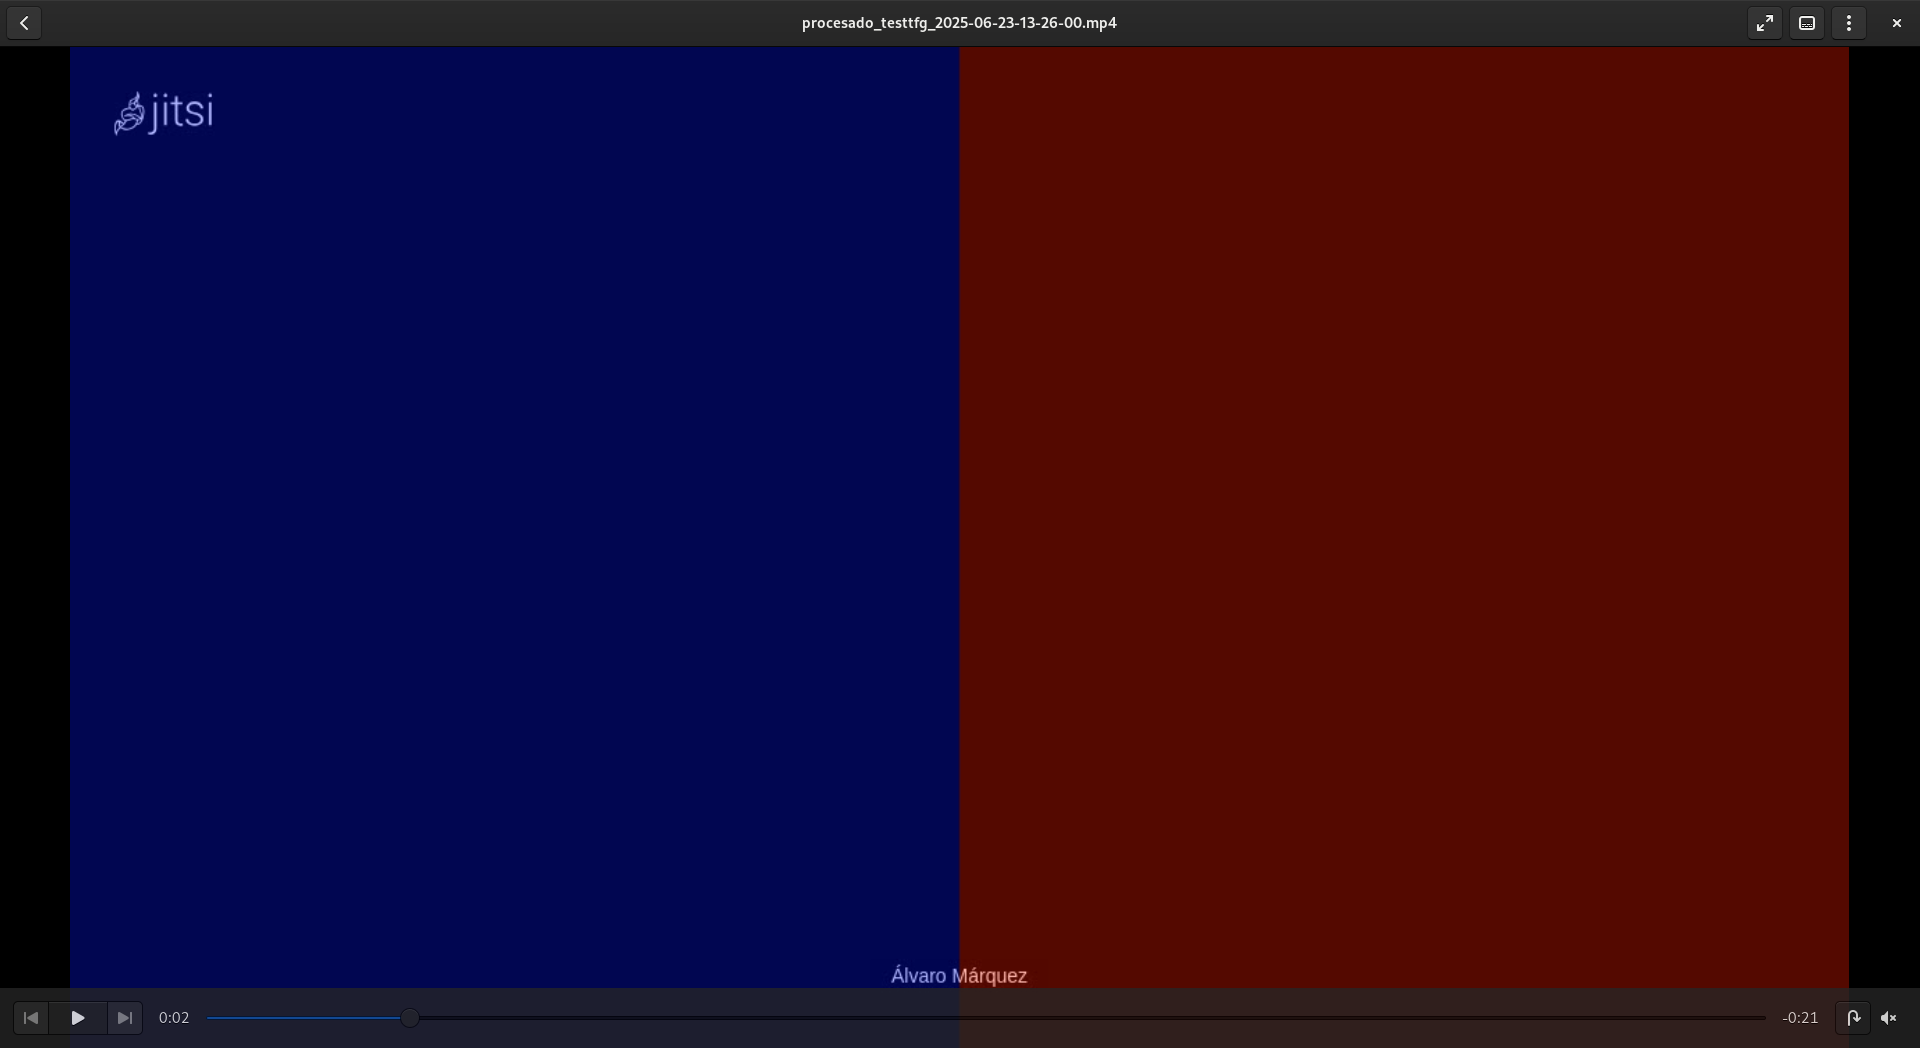
\includegraphics[width=0.9\textwidth]{img/resultado-procesamiento.png}
    \caption{Captura de video ya procesado.}
    \label{fig:prueba_funcional}
\end{figure}

\section{Fallos y Soluciones}
\label{sec:fallos_soluciones}
En este apartado se exponen algunos de los errores y desafíos técnicos más relevantes por los que se ha visto comprometido el proyecto a lo largo de su desarrollo. Se detalla para cada uno el síntoma observado, el diagnóstico técnico de la causa raíz y la solución final que se implementó.

\subsection{Fallo 1: Inestabilidad Crítica del Despliegue en Entorno Windows (WSL2)}
\begin{itemize}
    \item \textbf{Síntoma:} Inoperabilidad total de la pila \texttt{docker-jitsi-meet}. El \textit{log} del contenedor Prosody (servidor de autenticación) mostraba errores críticos y repetitivos de \texttt{Permission denied}. El contenedor Jibri no lograba arrancar o entraba en un bucle de reinicios, mostrando en sus logs errores de autenticación \texttt{SASLError}.
    
    \item \textbf{Diagnóstico Técnico:} Se determinó que existía un conflicto irresoluble en la traducción de permisos entre el sistema de ficheros de Windows (NTFS) y el de Linux (ext4) que usan los contenedores. La capa de virtualización de WSL2 no gestionaba adecuadamente los permisos de propietario/grupo (\texttt{chown}/\texttt{chgrp}) que los servicios de Jitsi necesitaban para operar.
    
    \item \textbf{Solución Aplicada:} Abandono completo del entorno Windows. Se realizó una instalación nativa de Debian 12, proporcionando un entorno de sistema de ficheros y permisos 100\% compatible, lo que se considera la solución estándar para despliegues de servidor robustos.
\end{itemize}

\subsection{Fallo 2: Despliegue de Jitsi en Debian - Errores de Conexión en Cascada}
\begin{itemize}
    \item \textbf{Síntoma:} Tras un despliegue exitoso en Debian, la interfaz web no permitía unirse a una sala, mostrando el error "La conexión ha fallado". La depuración reveló múltiples problemas encadenados: el cliente web intentaba una conexión segura (WSS) en un servidor HTTP, un posterior error de montaje \texttt{not a directory} al intentar forzar la configuración con \texttt{custom.config.js}, y finalmente un error de "Ha sido desconectado" al entrar en una sala.
    
    \item \textbf{Diagnóstico Técnico:} Se diagnosticaron tres problemas independientes: 1) una configuración por defecto del cliente que forzaba WSS; 2) la creación accidental de un directorio en lugar de un fichero de configuración en el \textit{host}; y 3) la falta de un \texttt{VirtualHost} en la configuración de Prosody para la autenticación de usuarios invitados.
    
    \item \textbf{Solución Aplicada:} Se solucionó cada problema de forma secuencial: se creó correctamente el fichero \texttt{custom.config.js} para forzar la conexión HTTP y, crucialmente, se modificó el fichero de configuración \texttt{jitsi-meet.cfg.lua} de Prosody para añadir la configuración del \texttt{VirtualHost} de invitados.
\end{itemize}

\begin{figure}[H]
    \centering
    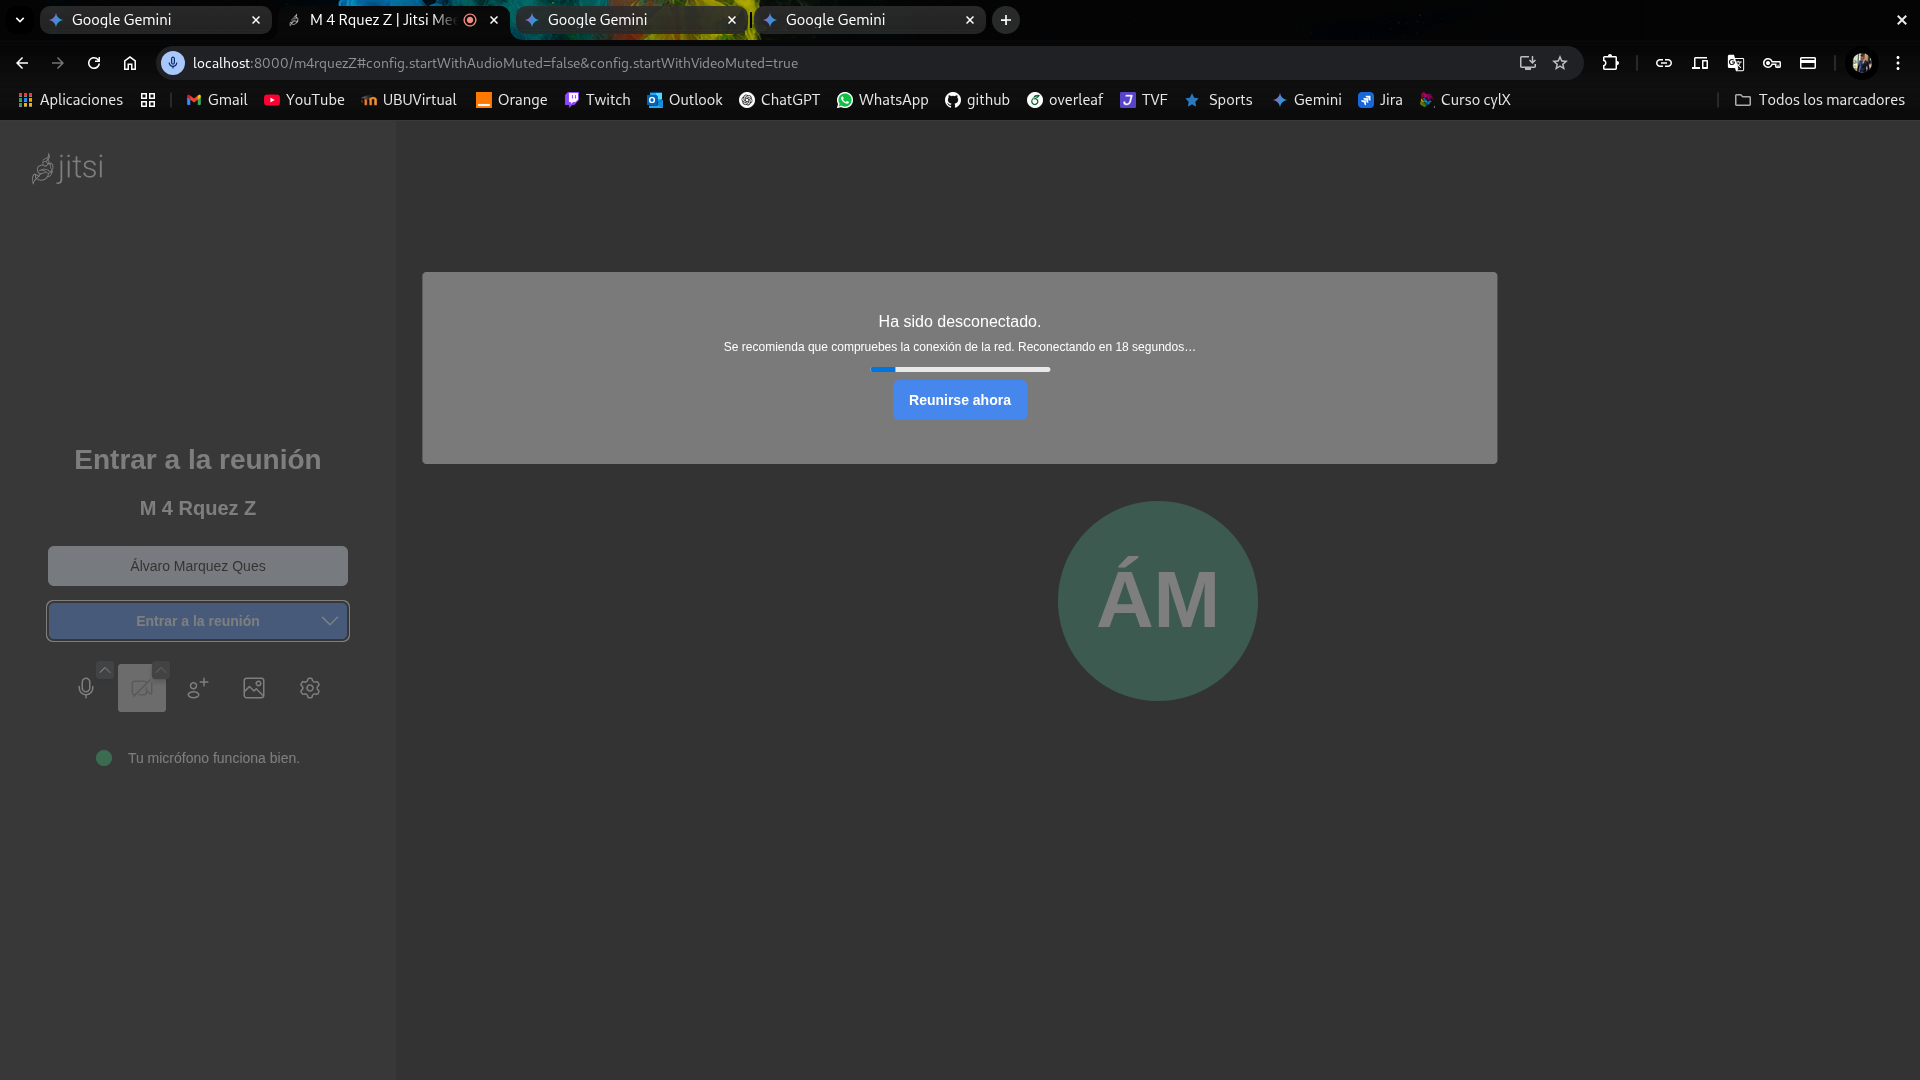
\includegraphics[width=0.9\textwidth]{img/errorconexion.png}
    \caption{Capture de error persistente de Conexión.}
    \label{fig:anexod_error_conexion}
\end{figure}

\subsection{Fallo 3: Problemas de Red para la Validación de Certificados SSL}
\begin{itemize}
    \item \textbf{Síntoma:} Al intentar implementar HTTPS con Let's Encrypt, el proceso de validación de certificados fallaba.
    \item \textbf{Diagnóstico Técnico:} Se determinó que los servidores de Let's Encrypt no podían alcanzar la máquina anfitriona en los puertos 80 y 443. Esto se debía a la naturaleza dinámica de la IP doméstica y a la falta de configuración en el \textit{router} local.
    \item \textbf{Solución Aplicada:} Se implementó una configuración de red completa: 1) Se configuró un DNS dinámico con \textbf{DuckDNS}. 2) Se asignó una IP local estática a la máquina Debian mediante reserva de DHCP en el router. 3) Se configuró la re-dirección de puertos (\textit{Port Forwarding}) en el \textit{router} para dirigir el tráfico de los puertos 80 y 443 a la IP fija de la máquina Debian.
\end{itemize}

\subsection{Fallo 4: Grabaciones de Jibri con Vídeo en Negro}
\begin{itemize}
    \item \textbf{Síntoma:} El servicio Jibri generaba un fichero \texttt{.mp4} del tamaño correcto, pero este estaba completamente en negro y sin sonido.
    \item \textbf{Diagnóstico Técnico:} El análisis de los \textit{logs} de Jibri (\texttt{(EE) no screens found(EE)}) reveló que el entorno gráfico virtual (Xvfb) no podía iniciarse. La causa raíz fue la falta del módulo del kernel \texttt{v4l2loopback} en el sistema anfitrión Debian, necesario para crear un dispositivo de vídeo virtual del cual grabar.
    \item \textbf{Solución Aplicada:} Se realizó la instalación del módulo requerido en el \textit{host} con el comando \texttt{sudo apt install v4l2loopback-dkms} y se reinició el sistema.
\end{itemize}

\subsection{Fallo 5: Errores Durante la Construcción de una Imagen Docker Personalizada}
\begin{itemize}
    \item \textbf{Síntoma:} Al intentar construir una imagen de Jibri personalizada para depurar, el proceso \texttt{docker build} fallaba con errores de \texttt{apt-get update}.
    \item \textbf{Diagnóstico Técnico:} Se identificaron dos problemas en el \texttt{Dockerfile} base: 1) una clave GPG expirada de un repositorio de Google Chrome y 2) la referencia a un paquete obsoleto (\texttt{libindicator3-7}).
    \item \textbf{Solución Aplicada:} Se modificó el \texttt{Dockerfile} para eliminar el fichero de repositorio problemático antes de ejecutar \texttt{apt-get update} y se reemplazó el paquete obsoleto por su sucesor, \\ \texttt{libayatana-appindicator3-1}.
\end{itemize}

\subsection{Fallo 6: Conflictos y Errores en el Pipeline de Spark}
\begin{itemize}
    \item \textbf{Síntoma:} Al levantar el pipeline de procesamiento, surgieron múltiples errores: un conflicto de puertos (8080), errores de importación en Python (`ModuleNotFoundError`, `numpy.core.multiarray failed to import`), una excepción `java.io.InvalidClassException`, una "condición de carrera" al conectar con Spark y un bucle de procesamiento infinito.
    \item \textbf{Diagnóstico Técnico:} Se diagnosticaron cinco problemas distintos: 1) Conflicto del puerto del Spark Master con el Jitsi Videobridge. 2) Falta de un fichero \texttt{requirements.txt} y un conflicto de versiones entre OpenCV y NumPy. 3) Incompatibilidad entre la versión de la librería PySpark y la imagen Docker de Spark. 4) El \textit{script} de Python intentaba conectar antes de que el máster de Spark estuviera listo. 5) El \textit{script} no tenía lógica para gestionar los vídeos ya procesados.
    \item \textbf{Solución Aplicada:} Se aplicaron soluciones específicas para cada problema: 1) Se cambió el puerto del Spark Master al 8081. 2) Se creó un \texttt{requirements.txt} fijando las versiones (\texttt{pyspark==3.5.0}, \texttt{numpy<2.0}). 3) Se fijó la versión de la imagen de Spark a \\(\texttt{bitnami/spark:3.5.0}. 4) Se añadió un retardo de 10 segundos \\ (\texttt{time.sleep(10)}) al inicio del \textit{script}. 5) Se implementó la lógica de mover el vídeo original a una carpeta \texttt{/archived} tras su procesamiento.
\end{itemize}
\apendice{Documentación de Usuario}
\label{apendice:manual_usuario}

\section{Introducción}
\label{sec:manual_intro}
Este manual proporciona una guía detallada para el despliegue y uso de la infraestructura de procesamiento de vídeo desarrollada en este TFG. El objetivo es ofrecer al usuario técnico (en adelante, el Administrador) todos los pasos necesarios para poner en marcha el sistema completo.

La infraestructura consta de dos sistemas modulares que se despliegan de forma independiente pero que trabajan de manera conjunta: un servidor de captura de vídeo (Jitsi) y un pipeline de procesamiento de datos (Kafka y Spark).

\section{Requisitos Previos del Sistema}
\label{sec:manual_requisitos}
Antes de comenzar, es fundamental asegurar que la máquina anfitriona (\textit{host}) cumple con los siguientes requisitos.

\subsection{Requisitos de \textit{Hardware}}
\begin{itemize}
    \item \textbf{CPU:} Se recomienda un procesador de 4 o más núcleos con soporte para virtualización (VT-x/AMD-V) habilitado en la BIOS/UEFI.
    \item \textbf{Memoria RAM:} Debido a la cantidad de servicios, se recomienda un mínimo de \textbf{16 GB de RAM}.
    \item \textbf{Almacenamiento:} Mínimo de 50 GB de espacio libre en disco.
\end{itemize}

\subsection{Requisitos de Software del Sistema Anfitrión (\textit{Host})}
\begin{itemize}
    \item \textbf{Sistema Operativo:} Se requiere una distribución de Linux. Todo el desarrollo y validación se ha realizado sobre \textbf{Debian 12 "Bookworm"}.
    \item \textbf{Software Base:} Es necesario tener instalados los siguientes paquetes a través del gestor de paquetes \texttt{apt}:
        \begin{itemize}
            \item \texttt{git}: para la clonación de los repositorios.
            \item \texttt{docker.io}: motor de contenedores Docker.
            \item \texttt{docker-compose-v2}: herramienta de orquestación (\textit{plugin} de Docker).
            \item \texttt{curl} y \texttt{openssl}: herramientas de diagnóstico de red.
        \end{itemize}
    \item \textbf{Módulo del Kernel para Jibri:} Para que el servicio de grabación Jibri funcione correctamente y no genere vídeos con pantalla en negro, es \textbf{crítico} instalar el siguiente módulo del kernel que crea un dispositivo de vídeo virtual:
    \begin{verbatim}
sudo apt update
sudo apt install v4l2loopback-dkms
    \end{verbatim}
    Tras la instalación, se recomienda reiniciar el sistema anfitrión.
\end{itemize}

\subsection{Requisitos de Red (para Jitsi)}
Para que el servidor Jitsi sea accesible desde internet y pueda obtener un certificado SSL/TLS válido, se necesita:
\begin{itemize}
    \item Un \textbf{nombre de dominio público}. Para este proyecto se utilizó un dominio gratuito de \textbf{DuckDNS}.
    \item Acceso al \textbf{\textit{router}} para configurar la \textbf{re-dirección de puertos} (\textit{Port Forwarding}) de los puertos TCP 80, TCP 443 y UDP 10000 hacia la IP privada de la máquina anfitriona.
\end{itemize}
(Recomendado) Asignar una dirección IP local estática a la máquina anfitriona en la configuración del \textit{router} (Reserva de DHCP). Esto asegura que la re-dirección de puertos no falle si la IP local del servidor cambia.

\begin{figure}[H]
    \centering
    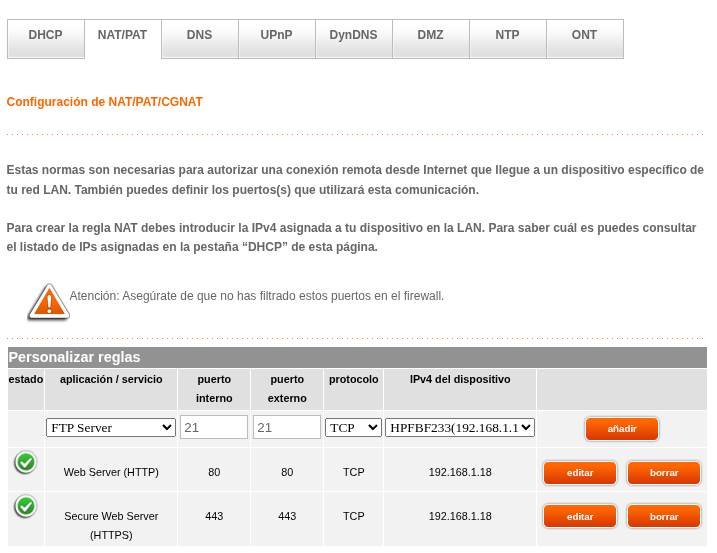
\includegraphics[width=0.9\textwidth]{img/routerconfig.png}
    \caption{Captura de configuración correcta personalizada puertos.}
    \label{fig:puertos_confi_anexoe}
\end{figure}
\begin{figure}[H]
    \centering
    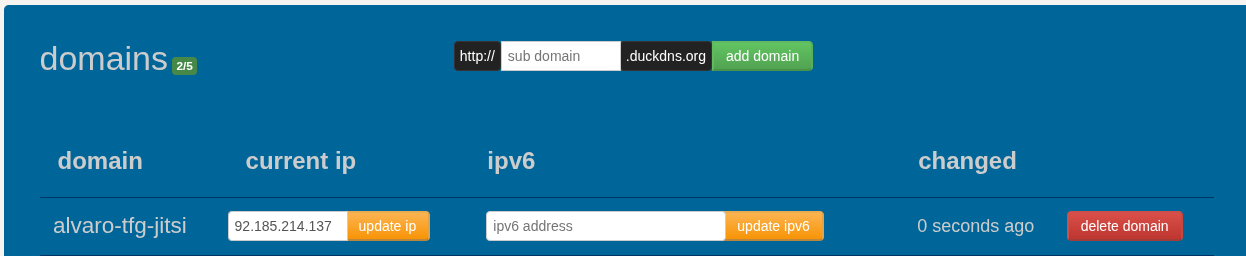
\includegraphics[width=0.9\textwidth]{img/duckdns.png}
    \caption{Captura de servicio Duckdns configurado.}
    \label{fig:duckdns_anexoe}
\end{figure}

\section{Instalación del Sistema}
\label{sec:manual_instalacion}
La instalación se divide en dos fases: el despliegue del servidor Jitsi y, posteriormente, el despliegue del pipeline de procesamiento.

\subsection{Fase 1: Despliegue del Servidor de Captura (Jitsi)}
\begin{enumerate}
    \item \textbf{Clonar el repositorio oficial de \texttt{docker-jitsi-meet}:}
    \begin{verbatim}
git clone https://github.com/jitsi/docker-jitsi-meet.git
cd docker-jitsi-meet
    \end{verbatim}

    \item \textbf{Copiar y configurar el fichero de entorno:} Se debe copiar el fichero de ejemplo y editarlo para ajustar los parámetros a nuestro entorno.
    \begin{verbatim}
cp env.example .env
nano .env
    \end{verbatim}
    Dentro del fichero \texttt{.env}, es crucial configurar las siguientes variables:
    \begin{itemize}
        \item \texttt{PUBLIC\_URL}: El dominio público que se utilizará \\(ej. \texttt{https://mi-tfg.duckdns.org}).
        \item \texttt{LETSENCRYPT\_DOMAIN}: El mismo nombre de dominio.
        \item \texttt{LETSENCRYPT\_EMAIL}: Un correo electrónico para la gestión de los certificados Let's Encrypt.
        \item Habilitar Jibri y la grabación: \texttt{ENABLE\_RECORDING=1},\\ \texttt{ENABLE\_LIVESTREAMING=0}.
    \end{itemize}

    \item \textbf{Generar contraseñas:} Se ejecuta el \textit{script} proporcionado para generar todas las contraseñas internas de los servicios.
    \begin{verbatim}
./gen-passwords.sh
    \end{verbatim}

    \item \textbf{Crear directorios de configuración persistente:}
    \begin{verbatim}
mkdir -p ~/.jitsi-meet-cfg/{web/letsencrypt,transcripts,prosody \ 
/config,prosody/prosody-plugins-custom,jicofo,jvb,jigasi,jibri}
    \end{verbatim}
    \textbf{Nota Importante sobre la Configuración Web:} Es crucial verificar que dentro del directorio ~/.jitsi-meet-cfg/web/ no se cree accidentalmente una carpeta/archivo llamada "\textit{custom.config.js}". Si fuera necesario modificar la configuración del cliente, se deberá crear un fichero de texto con ese nombre.

    \item \textbf{Levantar los servicios de Jitsi:} Se utiliza el siguiente comando para iniciar todos los contenedores, incluyendo Jibri.
    \begin{verbatim}
docker compose -f docker-compose.yml -f jibri.yml up -d
    \end{verbatim}
\end{enumerate}

\subsection{Fase 2: Despliegue del Pipeline de Procesamiento}
\begin{enumerate}
    \item \textbf{Clonar el repositorio del TFG:} En una carpeta diferente, se clona el repositorio principal del proyecto.
    \begin{verbatim}
git clone https://github.com/alvaromarquez1002/ \ 
TFG-SISTEMA-PROCESAMIENTO-VIDEO.git
cd TFG-SISTEMA-PROCESAMIENTO-VIDEO/src
    \end{verbatim}
    
    \item \textbf{Configurar el volumen de datos:} Es importante verificar que en el fichero \texttt{docker-compose.yml} de esta carpeta, el volumen del servicio \texttt{python-processor} esté correctamente mapeado al directorio donde Jibri guarda las grabaciones \\ (por defecto, \texttt{\textasciitilde{}/.jitsi-meet-cfg/jibri/recordings}).
    (Opcional) Para realizar pruebas de desarrollo sin depender de Jitsi, se puede comentar la línea del volumen de Jibri en el fichero docker-compose.yml y activar una línea alternativa como - ./data:/app/data para usar vídeos de prueba locales.

    \item \textbf{Levantar los servicios del pipeline:} Desde la carpeta \texttt{/src}, se ejecuta el siguiente comando. La opción \texttt{--build} asegura que la imagen Docker del procesador se construya con el código más reciente.
    \begin{verbatim}
docker compose up --build -d
    \end{verbatim}
\end{enumerate}

\section{Manual de Uso}
\label{sec:manual_uso}
Una vez desplegados ambos sistemas, el flujo de trabajo para capturar y procesar una sesión es el siguiente.

\subsection{Realizar una Grabación con Jitsi}
\begin{enumerate}
    \item \textbf{Acceder a la conferencia:} El Terapeuta y el Paciente acceden a la URL del servidor Jitsi (ej. \texttt{https://mi-tfg.duckdns.org}) desde sus navegadores web.

    \begin{figure}[H]
    \centering
    
\includegraphics[height=0.6\textheight]{img/entrarreunion.jpg}
    \caption{Pantalla de inicio de Jitsi Meet donde el usuario inicia la conferencia.}
    \label{fig:manual_entrar_reunion}
    \end{figure}
    
    \item \textbf{Iniciar la grabación:} Una vez en la sala, el Terapeuta hace clic en el botón de "Más acciones" (tres puntos verticales) y selecciona la opción "Iniciar grabación". Se le pedirá confirmación para iniciar la sesión.
    \begin{figure}[H]
    \centering
    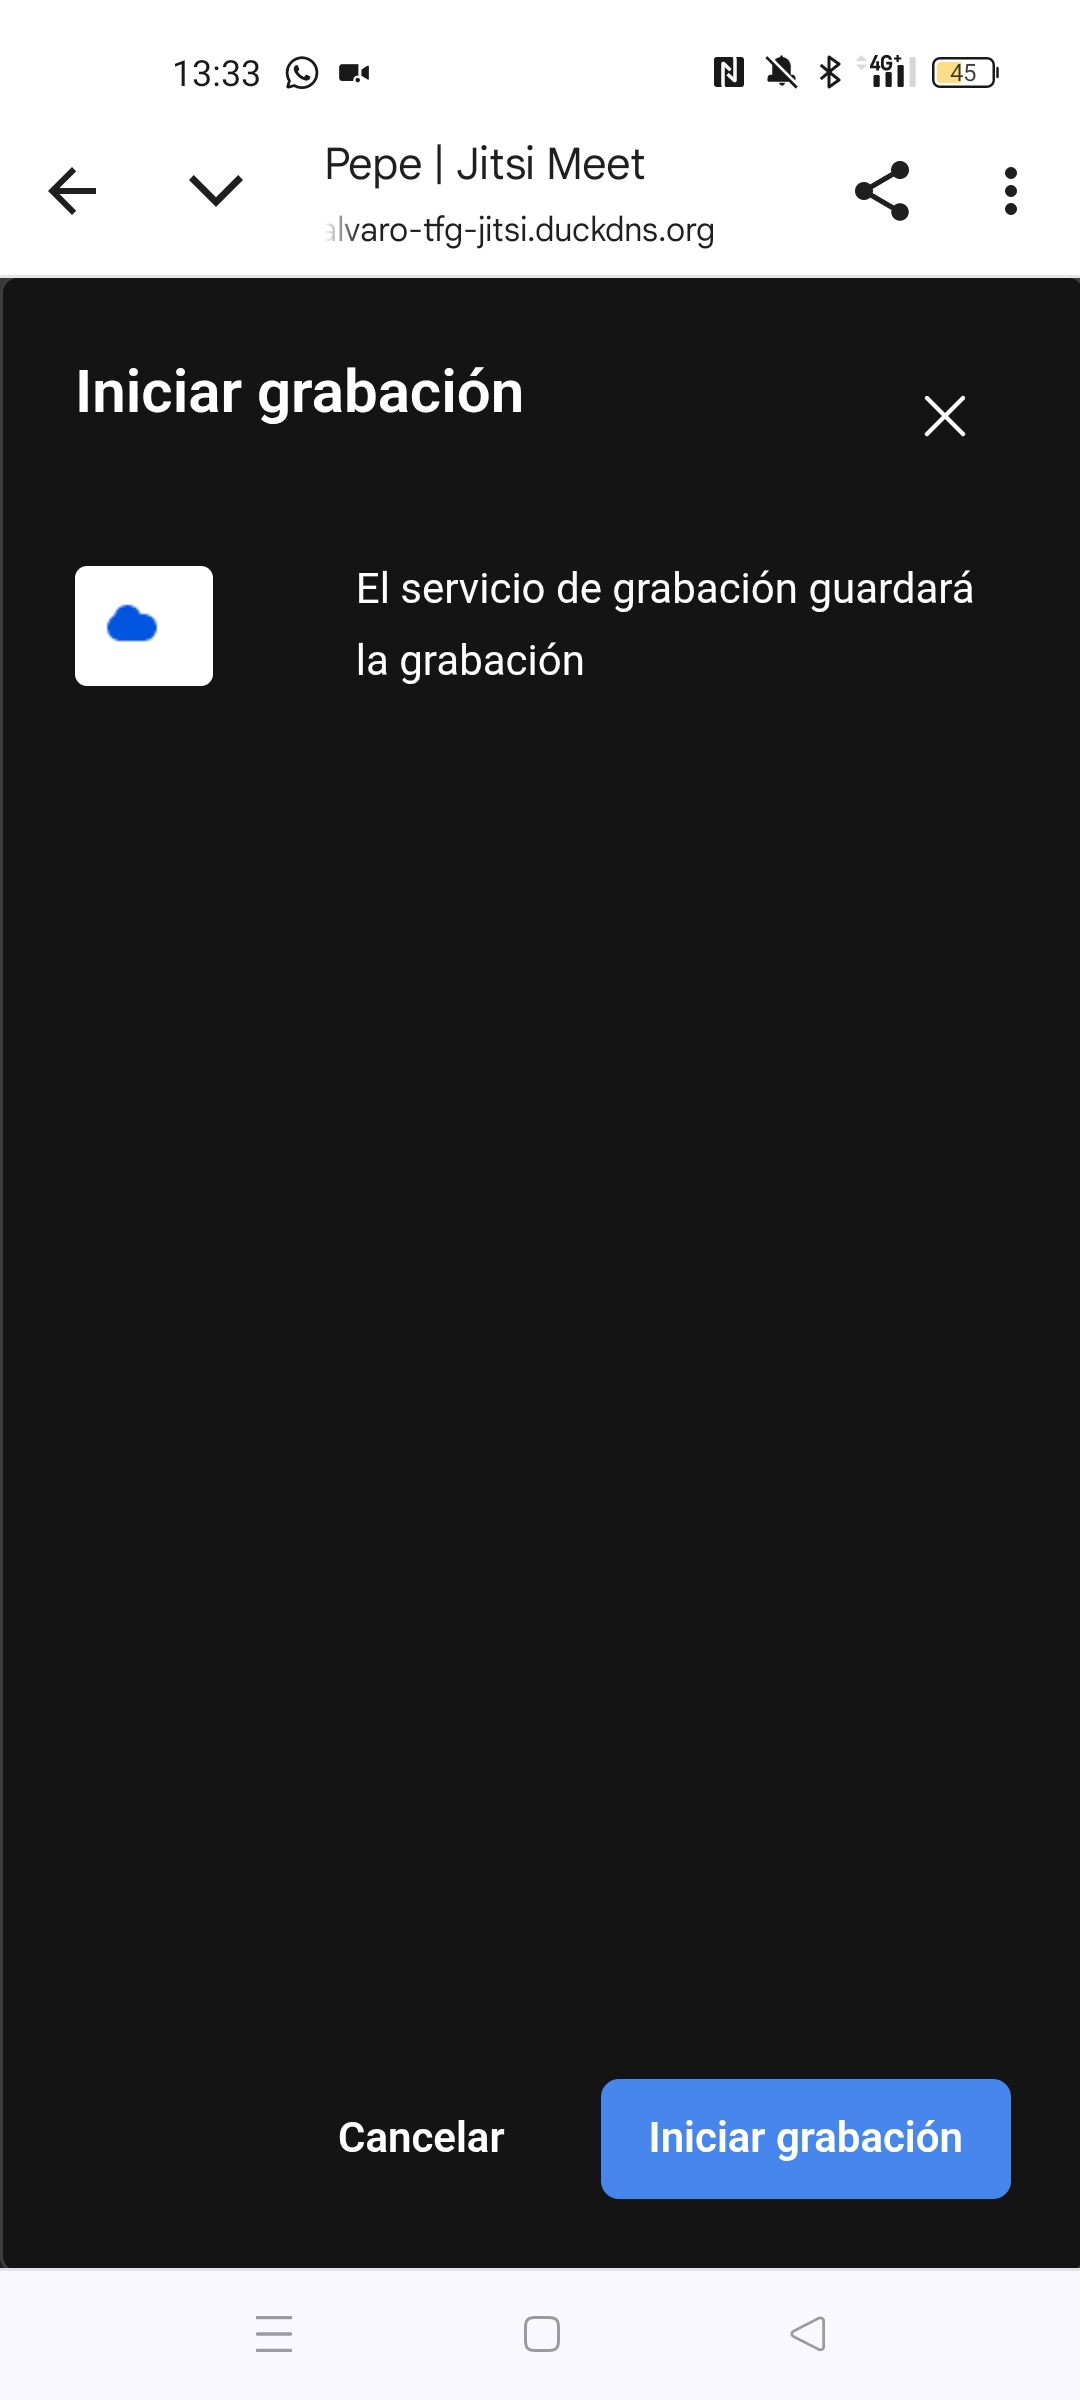
\includegraphics[height=0.6\textheight]{img/iniciargrabacion.jpg}
    \caption{Menú de opciones para iniciar la grabación de la sesión.}
    \label{fig:manual_iniciar_grabacion}
    \end{figure}
    
    \begin{figure}[H]
    \centering
    
\includegraphics[height=0.6\textheight]{img/grabacion.jpg}
    \caption{Indicador visual \textit{REC} que muestra que la sesión se está grabando activamente.}
    \label{fig:manual_grabando}
    \end{figure}
    
    \item \textbf{Detener la grabación:} Para finalizar, el Terapeuta repite el proceso y selecciona "Detener grabación".
\end{enumerate}

\subsection{Verificar el Vídeo Grabado}
Tras detener la grabación, el servicio Jibri tardará unos instantes en procesar y guardar el fichero.
\begin{enumerate}
    \item \textbf{Localizar el fichero:} El archivo MP4 resultante se guardará en el directorio del sistema anfitrión: \\ \texttt{\textasciitilde{}/.jitsi-meet-cfg/jibri/recordings/}.
    \item \textbf{Verificar contenido:} El Administrador puede reproducir este fichero para confirmar que el audio y el vídeo se han grabado correctamente. Este fichero es la entrada para el pipeline de procesamiento.
\end{enumerate}

\begin{figure}[H]
    \centering
    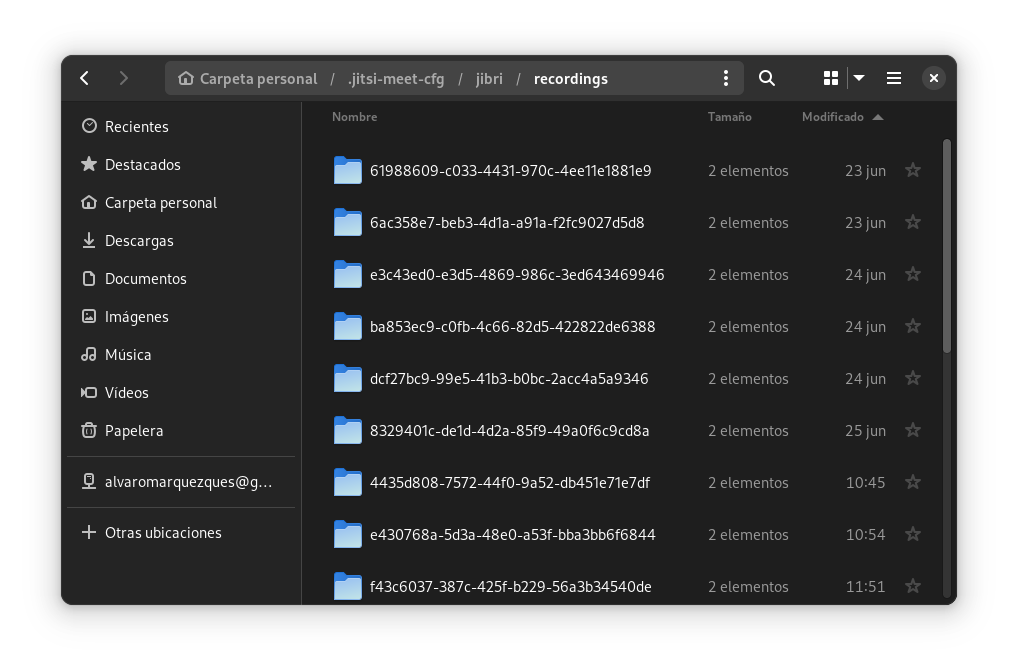
\includegraphics[width=\textwidth]{img/carpetarecordings.png}
    \caption{Ejemplo del directorio de grabaciones de Jibri con el fichero MP4 resultante.}
    \label{fig:manual_carpeta_grabaciones}
\end{figure}

\subsection{Ejecutar y Monitorizar el Procesamiento}
El pipeline de procesamiento está diseñado para ejecutarse de forma automática y continua.
\begin{enumerate}
    \item \textbf{Ejecución automática:} El \textit{script} \texttt{main.py} dentro del contenedor \texttt{python-processor} está constantemente buscando nuevos vídeos en el directorio de entrada.
    \item \textbf{Monitorizar el proceso:} Para ver el progreso en tiempo real, el Administrador puede ejecutar el siguiente comando en la terminal, desde la carpeta \texttt{/src} del proyecto:
    \begin{verbatim}
docker compose logs -f python-processor
    \end{verbatim}
    En la salida se podrán observar mensajes indicando qué vídeo se está procesando.
\end{enumerate}

\begin{figure}[H]
    \centering
    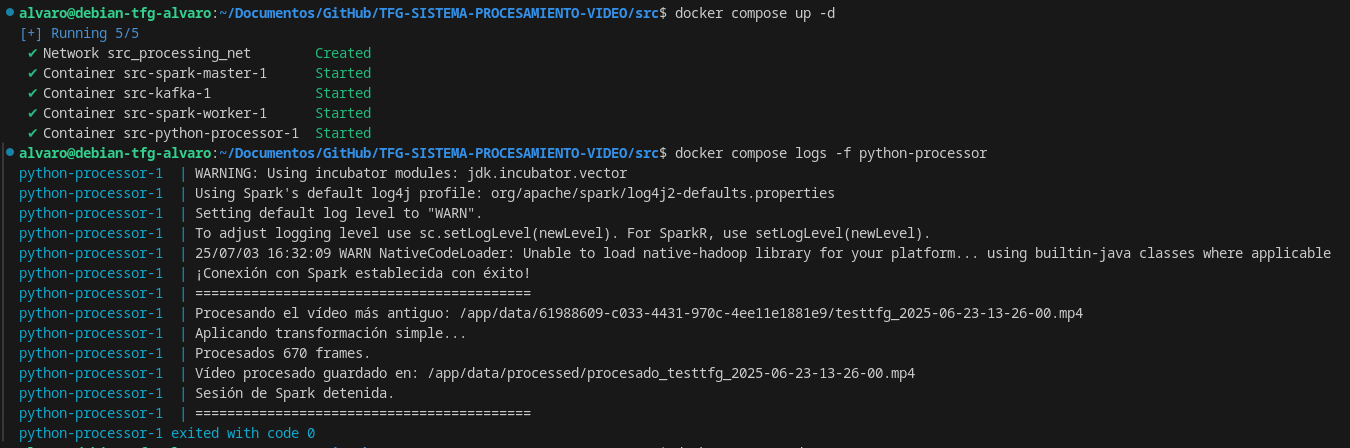
\includegraphics[width=\textwidth]{img/logsfinalpy.png}
    \caption{Monitorización de los logs del procesador Python, confirmando la ejecución del pipeline.}
    \label{fig:manual_logs_procesador}
\end{figure}

\subsection{Acceder al Resultado Final}
Una vez que el \textit{log} indica que el procesamiento ha finalizado, los resultados se pueden encontrar en las siguientes rutas (relativas a la carpeta del proyecto). El vídeo procesado aparecerá en la sub-carpeta /processed y el vídeo original será movido a la sub-carpeta /archived, ambas dentro del directorio donde se guardó originalmente la grabación (por defecto, ~/.jitsi-meet-cfg/jibri/recordings/):
\begin{itemize}
    \item \textbf{Vídeo procesado:} El nuevo vídeo con la transformación aplicada se encontrará en \texttt{/src/data/processed/}.
    \item \textbf{Vídeo original archivado:} El vídeo original que ha sido procesado se moverá a \texttt{/src/data/archived/} para evitar su procesamiento de nuevo.
\end{itemize}

\begin{figure}[H]
    \centering
    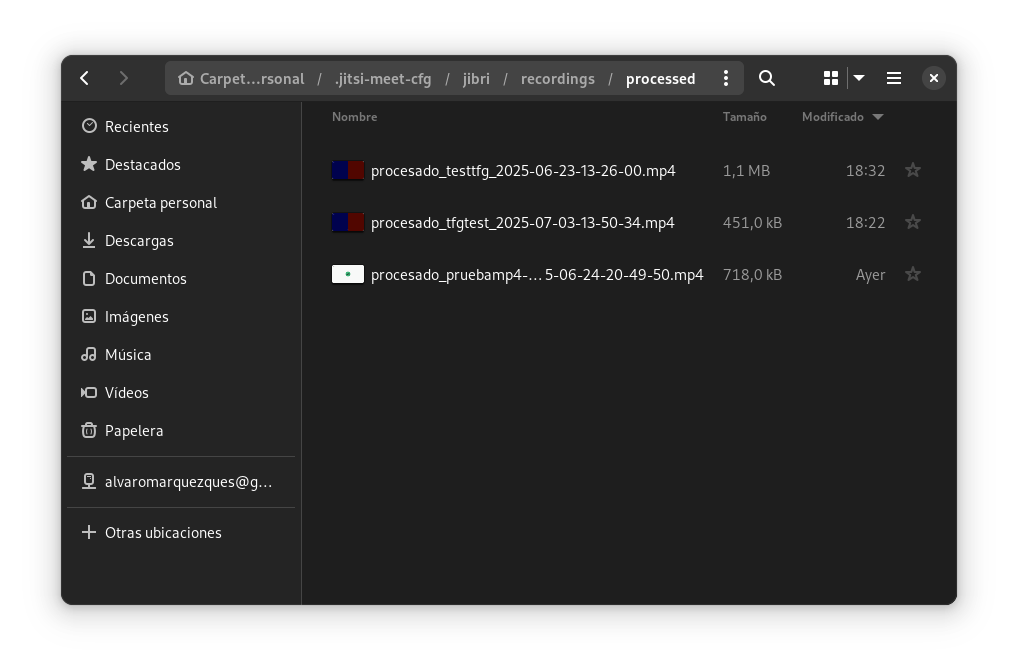
\includegraphics[width=\textwidth]{img/carpetaprocessed.png}
    \caption{Directorio de salida mostrando el vídeo final una vez procesado.}
    \label{fig:manual_carpeta_procesado}
\end{figure}

\section{Resolución de Problemas (FAQ)}
\label{sec:manual_faq}
\begin{itemize}

    \item \textbf{Problema:} No se puede acceder a la instancia de Jitsi desde internet.
    \item \textbf{Causa y Solución:} Verificar que el servicio de DNS dinámico \\ (DuckDNS) está apuntando a la IP pública correcta y que la re-dirección de puertos (80, 443) está bien configurada en el \textit{router}.

    \item \textbf{Problema:} El contenedor \texttt{python-processor} falla al iniciar con un error de conexión a Spark.
    \item \textbf{Causa y Solución:} Esto puede ser una "condición de carrera". El \textit{script} intenta conectar con Spark antes de que el clúster esté completamente listo. El \textit{script} incluye un retardo para mitigar esto, pero si el problema persiste, se puede probar a reiniciar únicamente el contenedor del procesador: \texttt{docker compose restart python-processor}.

    \item \textbf{Problema:} El \textit{log} del contenedor python-processor muestra un error "ModuleNotFoundError" o un conflicto de versiones con NumPy.
    \item \textbf{Causa y Solución:} Esto se debe a una incompatibilidad entre las librerías de Python. Asegúrese de que el fichero \texttt{requirements.txt} del procesador especifica las versiones correctas y compatibles (pyspark==3.5.0, numpy<2.0) y reconstruya la imagen con el comando \texttt{"docker compose up --build"}.

    \item \textbf{Problema:} Al intentar ejecutar un contenedor de Jitsi (especialmente Jibri) aparece un error "s6-mkdir: permission denied" incluso usando sudo.
    \item \textbf{Causa y Solución:} Este es un problema avanzado causado por una incompatibilidad entre el sistema de inicio s6-overlay de la imagen de Docker y el entorno del \textit{host}. La solución implementada en este TFG fue construir una imagen de Jibri personalizada desde un Dockerfile limpio para evitar el conflicto. Consulte la documentación técnica (Apéndice D) para más detalles sobre esta implementación.
    
\end{itemize}
\apendice{Anexo de sostenibilización curricular}

\section{Introducción}
Este anexo incluirá una reflexión personal del alumnado sobre los aspectos de la sostenibilidad que se abordan en el trabajo.
Se pueden incluir tantas subsecciones como sean necesarias con la intención de explicar las competencias de sostenibilidad adquiridas durante el alumnado y aplicadas al Trabajo de Fin de Grado.

Más información en el documento de la CRUE \url{https://www.crue.org/wp-content/uploads/2020/02/Directrices_Sosteniblidad_Crue2012.pdf}.

Este anexo tendrá una extensión comprendida entre 600 y 800 palabras.



\bibliographystyle{plain}
\bibliography{bibliografiaAnexos}

\end{document}
